%!TEX TS-program = xelatex
% !TEX root = ../thesis.tex
% Do not delete; used to set build system

%\begin{savequote}[75mm] 
%Nulla facilisi. In vel sem. Morbi id urna in diam dignissim feugiat. Proin molestie tortor eu velit. Aliquam erat volutpat. Nullam ultrices, diam tempus vulputate egestas, eros pede varius leo.
%\qauthor{Quoteauthor Lastname} 
%\end{savequote}

\chapter{Absolute protein quantitation: Inference with non-ignorable missing data in high throughput proteomics}
\label{proteomics:ch:proteomics}

\section{Introduction}
\label{proteomics:sec:intro}

Proteins are the leading actors in cellular processes, making them a prime target for biological investigation.
Understanding their absolute concentrations within a population of cells can elucidate the molecular dynamics that regulate their functions \citep{Ishihama:2005ir} and open a broad range of biological processes to deeper investigation.
However, measuring the concentration of many proteins in a single experiment has been difficult \citep{Ghaemmagham:2003tu}. 
As a result, many investigations have relied upon gene expression as a proxy for the concentration of these proteins \citep{Franks:2013}.
In recent years a new field of high-throughput proteomics has emerged, in which biologists and biochemists have begun exploring the next level of biological complexity with Fourier transform mass spectrometers  \citep{Scigelova:2006p10560,Scigelova:2011dt}.
High-throughput mass spectrometry can deliver a fine-grained view of cellular activity at an unprecedented scale and precision.
In principle, this new technology enables the direct estimation of absolute protein concentrations from the relative intensities of protein fragments in a biological sample.

In practice, the measurement process implemented by mass spectrometers introduces complex systematic biases that must be accounted for to obtain valid estimates of absolute protein concentrations.
Proteins are large macromolecules, consisting of intricately-folded sequences of amino acids. 
They are enzymatically digested into fragments, which are amenable to analysis by mass spectrometry \citep{Thakur:2011kz}. 
% Introduce distinction between fragments (unidentified peptides) and peptides (identified up to a modification or charge state).
Protein fragments are generally referred to as {\em peptides}; throughout this paper, fragments with the same sequence but distinct characteristics (e.g., charge states and chemical modifications) are considered {\em distinct} peptides. 
%A typical biological sample contains hundreds of thousands of peptides. 
These peptides are analyzed by two separate mass spectrometers to produce quantitative summaries \citep{Steen:2004tk}.
Because of sample complexity and instrument limitations, however, not all of the peptides can be analyzed in the second-stage of mass spectrometry to have their sequence identified.
The instrument is programmed to select the most abundant peptides in the first stage of mass spectrometry for sequencing, at any given time.
This multi-stage measurement process results in a systematic bias towards observing peptides from the sample's most abundant proteins.
In this paper, we present and evaluate a statistical technique to correct these biases, providing reliable estimates of absolute protein abundances from mass spectrometry experiments.

Figure \ref{proteomics:fig:Mass_Spec_Overview} illustrates the experimental process in detail.
%
\ifx\nofigures\undefined
\begin{figure}[t]
 \centering
% 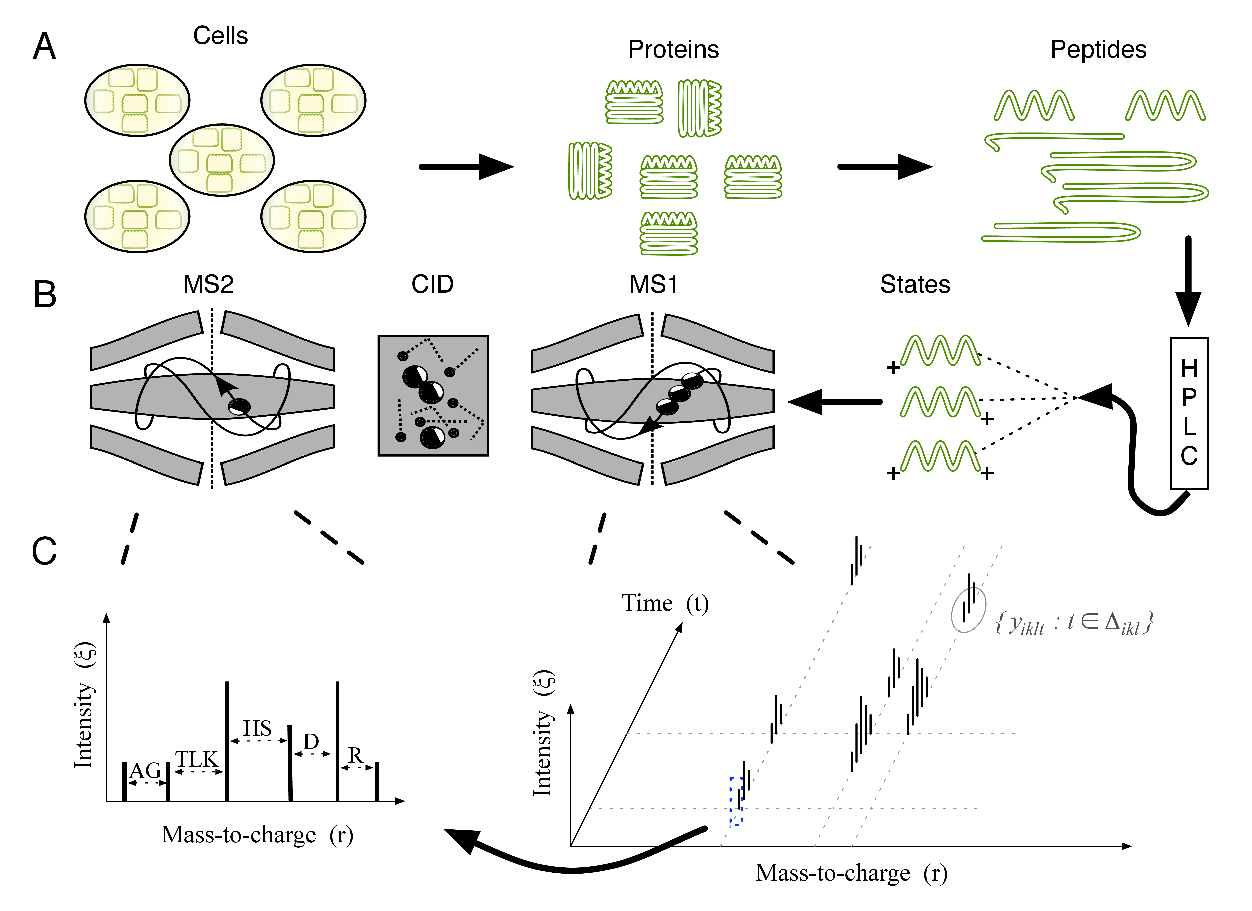
\includegraphics[width=\textwidth]{figures/proteomics/MS_Overview_small}
% \caption{MS proteomics overview. 
% (A) From cells to protein fragments. 
% (B) Fragments are separated in time, charged with ions, then analyzed using two mass spectrometers.
% (C) The HPLC separates the peptide
%mixture as well as determining the relative abundance of the mixture
%at each time point. MS1 determines the intensities of each compontent
%of the mixture at the given timepoint. Finally, the MS2 determines
%the sequence of a subset of peptide states.}
 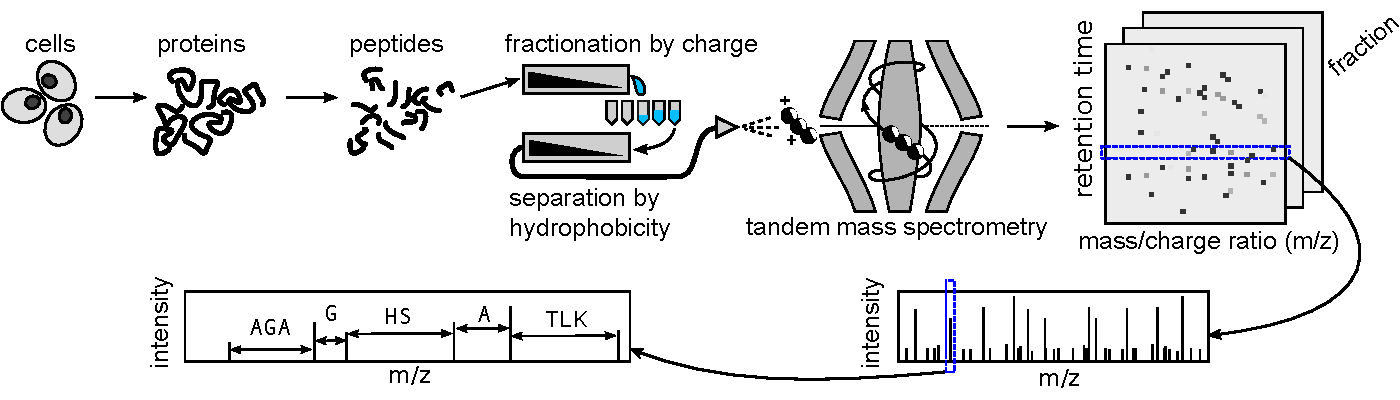
\includegraphics[width=\textwidth]{figures/proteomics/mass-spec-errors-awb}
 \caption{Overview of the measurement process in LC-MS/MS proteomics. 
 Clockwise from top left: Cells are lysed to extract proteins, which are broken down into fragments by a protease.
These fragments are then fractionated by charge and separated by hydrophobicity in the liquid chromotography (LC) stage before being sent through tandem mass spectrometry (MS/MS).
This yields the spectrographic intensity (shown by shaded dots) and mass/charge ratio for each fragment retention time.
A subset of these fragments are selected for further processing at each time, allowing for identification.
\label{proteomics:fig:Mass_Spec_Overview}}
\end{figure}
\fi
%
Starting from the top left, a culture of approximately $10^{8}$ cells are opened (lysed) to extract their proteins, which are then digested with an enzyme (protease) into fragments (peptides).
These peptides are then separated based on their hydrophobicity (via high-performance liquid chromatography).
As peptides reach the spray tip gradually, they are given an electrical charge and fly into the mass spectrometer.
All of these steps simply transform the long, complex mass of proteins from our cell culture into a well-separated set of simpler molecules that the mass spectrometers can process.

Fragments that are ionized within the same short time window are analyzed together by the first of two mass spectrometers (MS1).
At this stage, fragments with the same sequences of amino acids are present in a number of different states as a result of ion charges, \emph{in vivo} post-translational modifications and \emph{in vitro} chemical modifications from the sample preparation \citep{Michalski:2011gm}.
This step results in raw measurements $\xi(t, r)$ each of which quantifies the intensity\footnote{This intensity corresponds to the magnitude of a Fourier coefficient associated with peptides of mass-to-charge ratio $r$ \citep{Scigelova:2006p10560}. Modern mass spectrometers generally measure the amplitudes at which ionized protein fragments oscillate along an electrode over time. The Fourier transformation $\xi(f)$ of the amplitude time series from a mixture of ionized fragments provides the power associated with each frequency $f$. Each frequency $f$ is associated with fragments of a particular mass-to-charge ratio $r$ according to $f=C/r$, where $C$ encodes instrument geometry and settings, yielding $\xi(t, r(f)) = \xi(t, r)$.
% m/z in dalton/charge
% (obs m - true m)/(tr m)*1M in ppm
% f = k*B/(2*\pi*m/z) with f=axial freq, B=force of EM field, and m/z as above -- in orbitrap} %%% brief explanation of intensity %%%
}
%
corresponding to ionized fragments with mass-to-charge ratio $r$, analyzed within a time window indexed by $t$.
These intensities are proxies for relative abundance of fragment in the mass spectrometer within each time window.
%
The rightmost sections of Figure \ref{proteomics:fig:Mass_Spec_Overview} illustrate the output of this process, with each fraction yielding a set of intensities $\xi(t, r)$ for each (retention) time $t$ and mass-to-charge ratio $r$.
The lower right panel of this figure shows one slice through this dataset corresponding to a particular time $t$.
%
A subset of the fragments analyzed by the first mass spectrometers is selected, based on their intensities, to be broken down into yet smaller fragment components by collision with a gas.
The products of these collisions are then analyzed by a second mass spectrometer (MS2).
This step results in an additional set of intensity measurements for these components, each of which has a distinct mass-to-charge ratio and is associated with its original fragment's mass-to-charge ratio by the instrument.
The final (bottom left) panel of Figure \ref{proteomics:fig:Mass_Spec_Overview} shows the intensity spectrum obtained by MS2 for the components of the fragments with mass-to-charge ratio $r$ selected from MS1.
The amino acid sequence of these fragments can often be reliably determined by analyzing differences in the mass-to-charge ratio between adjacent peaks in the MS2 spectrum.
%Peptides with exactly the same mass-to-charge ratio and sequence bits cannot be distinguished, but this occurs quite rarely give the accuracy of the instrument (1-2 parts-per-million) and the combinatorial explosion in the number of peptides---possible fragments times possible ion charge states times possible post-translational and chemical modifications.

% two stat problems: identification/matching, absolute abundance estimation.

The statistical problem of interest is to estimate the absolute concentrations of proteins in a sample from the observed peptide-level intensities $\{\xi(t, r):t\in T,r\in R\}$.
However, to tackle this problem, we must first associate these raw intensities with peptides and condense them into a more manageable set of summaries.
This preprocessing falls under the heading of identification, a well-studied problem in MS/MS proteomics.
%
In the identification task, the intensity and mass-to-charge data from MS2 are used to detect which peptides are present in the sample, in terms of their most likely sequence, charge, and possible chemical and post-translational modifications.
In a typical run, hundreds of thousands of unique peptides are simultaneously detected.
The observed spectrum of each detected peptide is then compared to the theoretical spectra of the all peptides that would be generated by digesting the proteins in the sample with a specific enzyme.
For example, the enzyme trypsin digests the amino acids arginine (R) and lysine (K), so each protein is expected to be fragmented into peptides by removing all arginines and lysines from its amino acid sequence.
Currently, several well-established methods for peptide/protein identification exist in the literature \citep{Cox:2008uu,Perkins:1999ed,Eng:1994fj}; we generally use the MaxQuant software of \citet{Cox:2008uu}.

Identification yields a set of integrated log-intensities $y_{ikl}^{obs}$, each of which is associated with peptide $k$ from protein $i$, and $l$ indexes distinct modifications and charge states.
These integrated log-intensities are known to be approximately linearly related to the log of the number of molecules of that peptide present in the mass spectrometer, making them an excellent basis for absolute quantitation \citep{Old:2005jf,Scigelova:2011dt}.
Formally, each $y_{ikl}$ is the result of two operations: a mapping between identified fragment and a given set of values for $(t, r) \in \Delta_{ikl}$, and the integration of $\xi(t,r)$ over these values.
%
The mapping serves to associate each observed $\xi(t, r)$ with a given peptide state $ikl$.
The raw intensities $\xi(t, r)$ are then integrated over a small window in both retention time and mass-to-charge ratio.
The former accounts for the fact that any given peptide $ikl$ is typically observed across adjacent time windows, while the latter accounts for minor variation in $r$ for each fragment originating from the presence of multiple isotopes and other factors.
Thus, all of our inferences are based on
%
\begin{equation}
y_{ikl}^{obs} = \log_{10}\left( \int \! \int_{(t, r) \in \Delta_{ikl}} \xi(t, r) \dd r \dd t \right) .
\end{equation}

With these quantities in-hand, we can refine the statement of our statistical problem: using the collection of integrated log-intensities $y_{ikl}^{obs}$ and known properties of the observed proteins, estimate the log-absolute concentrations of proteins in our sample $\zeta_i$.
We present a probabilistic model for these data in Section \ref{proteomics:sec:model}, with particular details of the core estimand $\zeta_i$ provided in Section \ref{proteomics:sec:estimand}.



\subsection{Related work}

There are two threads of literature on protein quantitation: relative and absolute quantitation. 
In relative quantitation, the estimand of interest is the ratio of a given protein concentration in two distinct samples  (generally different experimental conditions).
In contrast, absolute quantitation requires the ability to estimate the concentration of all proteins in a single sample, relative to one another---these quantities together with the total amount of protein measured in the sample lead to the estimand of interest in this work, $\{\zeta_i:i\in I\}$, as we discuss in Section \ref{proteomics:sec:estimand}.


While there has been much work on the problem of peptide identification \citep[e.g.,][]{Cox:2008uu,Perkins:1999ed,Eng:1994fj}, less progress has been made on the quantitation problem \citep{Makawita:2010eg}.
Despite the relatively strong correlation between the amount of each protein in a sample, the observed intensities, and the number of its peptides identified by the mass spectrometer \citep{Old:2005jf}, heterogeneity in this relationship between labs, samples, and even peptides from a common protein has hampered the development of robust quantitation methods \citep{Tabb:2010bc,Bell:2009il}.
To control for these sources of variation, the popular methods for relative quantitation rely on physically labeling each sample being compared, analyzing them simultaneously, and estimating the relative abundance protein-by-protein based on summaries of peptide intensity ratios \citep{Ong:2002tf}.
%
Existing experimental methods for estimating absolute abundance are quite intricate.
For each protein of interest, the experimenter must synthesize a set of synthetic, standard peptides.
They then compare the observed intensities of peptides from the sample to the intensities of the corresponding standard peptides, which are introduced at known concentrations \citep{Gerber:2003kq}.
These approaches have limited throughput, are experimentally complex, and are limited to quantitation of a preselected set of proteins.

Motivated by the limitations of experimental quantitation methodologies, there has been a growing interest in computational methods for relative and absolute quantitation.
The simplest of these are based on spectral counting, either in the form of ratio-based estimates for relative quantitation \citep{Liu:2004hv}, or using rescaled counts for absolute quantitation \citep{Ishihama:2005ir}.
More recently, a semi-supervised absolute quantitation method called APEX has been developed, which uses a large training dataset to learn how differences in physiochemical properties affect the probability of peptide identification, independent of abundance \citep{Lu:2006p10143}.
It then uses these estimated probabilities of identification to construct a weighted estimator of protein abundance.
%
Another class of methods uses peptide intensities, which have a wider dynamic range than spectral counts, for quantitation, the most common of which are based on simple summaries of observed intensities, such as their median \citep{deGodoy:2008jk, Silva:2005cn}.
Most recently, a few attempts have been made to combine intensity and identification information, for example using principle component analysis to combine these features across samples \citep[e.g.,][]{Dicker:2010ea}.
Finally, the most sophisticated techniques, which motivated our own work, are model-based methods for relative quantitation that account for missing data at the peptide level \citep{Karpievitch:2009wb,Luo:2009ff}.
However, by focusing on peptide-level missingness, these methods fail to account for the true amount of missing data, since each peptide is generally found in a number of different states, due to biological and chemical modifications \citep{Michalski:2011gm}.

%This is due, in part, to the misconception that the measurements produced by the mass spectrometer are extremely accurate and thus there is no need for any statistics after identification. This argument, however, is flawed. It ignores the selection bias implemented at multiple data collection stages within the instrument.
%This bias is especially significant for peptides and proteins present at low concentrations.
%In our work, we proposed a modeling framework that is able to account for and mitigate the selection bias. 
%
%Most of the existing literature is devoted to the relative quantitation task.
%In this case, the consequences of selection bias are arguably mitigated, at least from an empirical perspective.
%Because of this, the most popular methods available for relative quantitation do not involve statistical modeling.
%Rather, they are based on observable summaries produced by the identification procedures, for example spectral counting \citep{Liu:2004hv} and median intensity \citep{deGodoy:2008jk,Silva:2005cn}.
%As we show in Section \ref{proteomics:sec:empirical}, these methods perform poorly when adapted to the task of absolute quantitation as the estimates often span a limited range of absolute concentrations \citep{Schulze:2010fk}.
%
%There are only a handful of model-based methods for either absolute or relative quantitation, and they take very different approaches.
%A semi-supervised approach called APEX uses a training set of proteins to learn the physicochemical properties of peptides that influence their likelihood of detection, which is then used to compute the absolute abundance based on the number of peptide identifications weighted for their "detectability" \citep{Lu:2006p10143}.  More recently, a similar approach has been suggested that relies on principal component analysis and a kernel ... \citep{Dicker:2010ea}.
% An alternative approach relies on a different experimental protocol and technology, but ... \citep{Luo:2009ff}.
% Perhaps closest to our approach, \citet{Karpievitch:2009wb} develop a model that posits a non-ignorable observation model.
%The observation model is specified on peptide-level intensities.
%We show that there is little information at the peptide-level about the censoring process that can be leveraged to correct for the selection bias.
%Instead, our model specifies the observation model in terms of the intensities of peptides in different charge and chemical modification states, a level of measurement where  information about the selection bias can be found in the shared number of states among peptides present a high and low concentrations in the sample.
%Generally, existing methods for absolute quantitation also suffer from limited range of the estimated concentrations \citep{Schulze:2010fk}.

\subsection{Contributions of this article}

In this paper, we introduce a statistical model that combines a hierarchical intensity model with an observation model for intensity-based censoring, in Section \ref{proteomics:sec:model}.
This combination accounts for key aspects of the biology and of the data acquisition process, including the fact that peptides are observed in multiple charge and modification states, and that there are at least two missing data mechanisms that compound throughout any LC-MS/MS instrument.

Our approach is novel in a number of ways: 
 (1) the focus is on absolute, rather than on relative quantitation;
 (2) while most existing approaches to quantitation involve simple summary statistics after identification, we posit and estimate a realistic censoring mechanisms that results in non-ignorable missing data;
 (3) the model explains the variability in the  intensities of peptides observed in multiple charge and modification states, rather than the aggregated intensities for individual peptides.  
%
We find that accounting for non-ignorable missing data helps reduce the selection bias induced by the measurement process.
In addition, modeling intensity-based censoring at the level of peptide states helps transfer information from abundant to rare proteins, since the number of states we expect to observe any given peptide in is independent of abundance.
As we show in Sections \ref{proteomics:sec:simulations} and \ref{proteomics:sec:empirical}, these aspects of the model allows robust, accurate estimation of absolute protein abundances in complex samples with concentrations spanning many orders of magnitude. 

We provide efficient inference for this model, in Section \ref{proteomics:sec:estimation}, by leveraging a combination of Halley's method, adaptive Gauss-Hermite quadrature, and explicit envelopes for sampling the number of censored peptide states and the censored intensities.
In Section \ref{proteomics:sec:simulations}, we explore the frequentist coverage of interval estimates, and we compare the performance of the proposed method with existing methods for estimating absolute protein concentrations, as we systematically vary the abundance and the length of the target proteins.
In Section \ref{proteomics:sec:empirical}, we explore the extent to which key assumptions of our model hold in practice, and we analyze estimates based on three biological samples, processed with different LC-MS/MS settings, in which a set of proteins with known concentration was introduced for validation purposes.


 %%% %%% %%%
 %%% %%% %%%


\section{Model}
\label{proteomics:sec:model}

We develop a probabilistic model for the measurements, $y_{ikl}^{obs}$, the output of an LC-MS/MS experiment combined with identification analysis with standard software.
%This includes both the non-ignorable missing data mechanism induced these experimental techniques and the hierarchical structure of our observations.
The observed data consists of: the observed state-level intensities $y_{ikl}^{obs}$, indexed by protein $i$, peptide $k$, and charge state $l$, and the observed counts of observed states by peptides $s_{ik}^{obs}$.
We also know the number of possible peptides per protein $m_i$, for a given enzyme used for digestion, which is independent of the sample in theory but requires careful preprocessing in practice.

We are interested in inferring the abundance of each protein $i$ within the given sample.
This abundance is a monotone function of the parameter $\mu_i$ as detailed in Section \ref{proteomics:sec:estimand}. We posit the following model,
%
\begin{align}
%1 / \tau_i^2 &\sim \text{Gamma}(\alpha_\tau, \beta_\tau) \\
%1 / \sigma_i^2 &\sim \text{Gamma}(\alpha_\sigma, \beta_\sigma) \\
 \gamma_{ik}\mid\mu_{i}, \tau_{i}^2  &\sim \hbox{Normal}(\mu_{i},\tau_{i}^{2}), \, i=1,\ldots,n, \, k=1,\ldots,m_i \\
 s_{ik} \mid \lambda, r  &\sim 1+\hbox{ Negative-Binomial }(1-\lambda,r), \, k=1,\ldots,m_i \\
 y_{ikl} \vert \gamma_{ik}, \sigma_{i}^2   &\sim \hbox{Normal}(\gamma_{ik},\sigma_{i}^{2}), \, l=1,\ldots,s_{ik}\\
 R_{ikl} \vert \pi^{rnd}, s_{ik} &\sim \hbox{Bernoulli}(1 - \pi^{rnd}), \, l=1,\ldots,s_{ik} \\
 I_{ikl} \vert y_{ikl}, \bm \eta, s_{ik}, R_{ikl}=1 &\sim \hbox{Bernoulli}(1 - g(y_{ikl}; \bm \eta)), \, l=1,\ldots,s_{ik} \\
 O_{ikl} &= R_{ikl} \cdot I_{ikl} \\
 Y_{obs} &= \{y_{ikl} : O_{ikl} = 1\} \\
 Y_{mis} &= \{y_{ikl} : O_{ikl} = 0\}
\end{align}
%
This model consists of two pieces: the distribution of the complete data $Y_{com} = (Y_{obs}, Y_{mis})$ given the parameters, and the distribution of the observed data given the complete data and parameters.
Starting with the complete data for protein $i$, this model specifies that each peptide gets a mean intensity $\gamma_{ik}$ distributed around the protein-mean $\mu_i$. No prior distribution on $\mu_i$ is assumed.
Similarly, each state-level intensity $y_{ikl}$ is distributed around the peptide-level intensity.
The variances of these distributions are $\tau^2_i$ and $\sigma^2_i$ are drawn from inverse-Gamma distributions.
%
\begin{align}
1 / \tau_i^2 &\sim \text{Gamma}(\alpha_\tau, \beta_\tau) \\
1 / \sigma_i^2 &\sim \text{Gamma}(\alpha_\sigma, \beta_\sigma)
\end{align}

This is a straightforward Normal hierarchical model except for one complication.
%
The number of states per peptide $s_{ik}$ is drawn from a shifted negative binomial distribution.
This distribution is fixed across proteins and peptides, reflecting the physical independence between the number of possible charge states and a protein's abundance.
This invariance plays a crucial role in our inference, as we discuss in Sections \ref{proteomics:sec:estimation} and \ref{proteomics:sec:remarks}.
Hence, we have
\begin{align}
\label{proteomics:eq:complete_data_likelihood}
P(Y_{com} | \bm \mu, \bm \sigma^2, \bm \tau^2, r, \lambda) =
\prod_{ik} \Bigg[& \frac{1}{\tau_i} \phi\left( \frac{\gamma_{ik} - \mu_i}{\tau_i} \right)
\begin{pmatrix} s_{ik} + r - 2 \\ s_{ik} - 1 \end{pmatrix} \lambda^{r} (1 - \lambda)^{s_{ik} - 1} \cdot \\
\nonumber
& \prod_{l=1}^{s_{ik}} \left[ \frac{1}{\sigma_i} \phi\left( \frac{y_{ikl} -  \gamma_{ik}}{\sigma_i} \right) \right] \Bigg],
\end{align}
where $\phi(z)$ is defined as $\frac{1}{\sqrt{2 \pi}} \exp\left( -\frac{1}{2} z^2 \right)$.


 %%% %%% %%%

\subsection{Missing data mechanism}
\label{proteomics:sec:mdm}

The missing data mechanism operates at the state level and is characterized using two random variables.
The first is a random censoring indicator, $R_{ikl} \sim \text{Bernoulli}(1 - \pi^{rnd})$, which accounts for censoring due to factors other than abundance.
The second is an intensity censoring indicator, $I_{ikl} \sim \text{Bernoulli}(1 - g(y_{ikl}; \bm \eta))$, which accounts for the intensity-dependent censoring.
We assume $I_{ikl}$ is drawn only if $R_{ikl} = 1$, as shown in Figure \ref{proteomics:fig:Missing_Data_Indicators_Tree}.
%
\ifx\nofigures\undefined
\begin{figure}[ht!]
\begin{center}
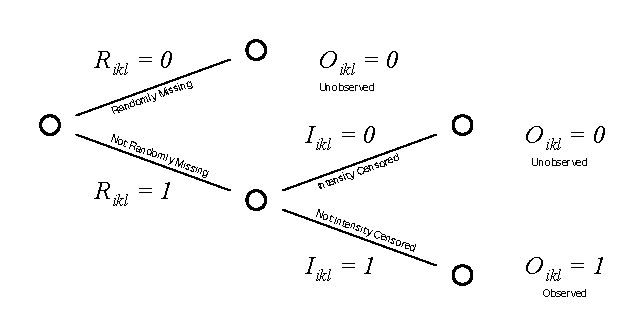
\includegraphics[width=.75\textwidth]{figures/proteomics/fig_tree_awb.pdf}
\end{center}
\caption{Possible missingness indicator values.\label{proteomics:fig:Missing_Data_Indicators_Tree}}
\end{figure}
\fi
%
Hence, we have
\begin{equation}
P(\bm I, \bm R | Y_{com}, \eta, \pi^{rnd}) =
\prod_{ikl} (\pi^{rnd})^{1 - R_{ikl}}
(1 - \pi^{rnd})^{R_{ikl}}
(1 - g(y_{ikl}; \eta))^{I_{ikl} R_{ikl}}
g(y_{ikl}; \eta)^{(1 - I_{ikl}) R_{ikl}},
\end{equation}
%
which implies a corresponding distribution on the (redundant) variables $\bm O \equiv \bm I \circ \bm R$, where $\circ$ denotes element-wise product, which indicate whether each intensity $ikl$ is observed.
In particular, the marginal probability of observing a given peptide state given $y_{ikl}$ and all other parameters is then
%
\begin{equation}
P(O_{ikl} = 1 | y_{ikl}, \bm \Theta) = (1 - \pi^{rnd}) (1 - g(y_{ikl}; \bm \eta)).
\end{equation}
%
In combination with (\ref{proteomics:eq:complete_data_likelihood}), these assumptions imply that
\begin{equation}
s_{ik}^{obs} | \bm \gamma, \bm \sigma^2, \bm s \sim \text{Binomial}(s_{ik}, (1-\pi^{rnd})(1 - \pi^{int}_{ik}))
\end{equation}
are conditionally independent across peptides, 
%%% EDO : YOU MEAN "ARE INDEPENDENT" ?? OF WHAT ??
%%% AWB : Conditionally independent across peptides
where $\pi^{int}_{ik} = \int_{\mathbb{R}} g(t; \eta) \frac{1}{\sigma_i} \phi\left( \frac{t - \gamma_{ik}}{\sigma_i} \right) \text{d}t$.
From this, we see how the division of the missing data mechanism into random and intensity-based censoring adds flexibility to our model, allowing the probability of missingness to asymptote to a value lower than 1 as intensity increases.
However, it is important to note that this separation is largely conceptual, not physical.
The random and intensity-based censoring mechanisms corresponds only roughly to the early and late stages of the LC-MS/MS process, respectively.

From a theoretical perspective, this missing data mechanism induces a stochastic dominance relationship between the distribution $Y_{obs}$ and $Y_{com}$, as Theorem \ref{proteomics:thm:dominance} establishes:
%
\begin{theorem}\label{proteomics:thm:dominance}
Suppose $X \sim F_X(x)$; that is, $X$ has a cumulative distribution function that can be represented as a Riemann-Stieltjes integral over $\mathbb{R}$. Let $Z | X=x \sim \Bernoulli( g(x) )$, where $g(x)$ is strictly increasing on $\mathbb{R}$ from $0$ to $1$. Then, the posterior distribution of $X$ given $Z=1$ stochastically dominates the original distribution of $X$.
\end{theorem}
%
This result establishes that observed intensities will be biased upwards relative to the complete ones.
We use this result for model checking in Section \ref{proteomics:sec:checkassumptions}. A proof is provided in Appendix \ref{proteomics:sec:proof1}.


 %%% %%% %%%

\subsection{Estimands}
\label{proteomics:sec:estimand}

The $\mu_i$ parameters are the primary target of the inference; however, they are not directly interpretable as absolute measures of protein abundance.
To provide absolute measures, we must convert $\mu_i$ from the log-intensity scale to the scale of protein abundances.
We define an estimand $\zeta_i$ for this purpose, 
%
\begin{equation}
\zeta_i = \log_{10} \left( \frac{T \times 10^{\mu_i}}{ \sum_{i=1}^{n} 10^{\mu_i}} \right) = \mu_i + \log_{10}(T) - \log_{10}\left(\sum_{i=1}^{n} 10^{\mu_i}\right), \label{proteomics:eq:abs_abund_estimand} 
\end{equation}
%
where $T$ is the total amount of proteins in the sample of interest.
The key feature of this estimand is normalization by $\sum_{i=1}^n 10^{\mu_i}$, which provides the core conversion from log-intensities to the log-abundance scale (up to an additive constant).
The total protein amount $T$ serves primarily as a rescaling factor for interpretability, which converts estimates from log-proportion of proteins to log-molecules per cell or log-femtomoles. 
We assume that $T$ is known and fixed. While this assumption is often challenged in practice, it is crucial to neither the validity nor the utility of our estimates. Modeling $T$ is also a possibility.

 %%% %%% %%%
 %%% %%% %%%


\section{Inference and estimation}
\label{proteomics:sec:estimation}

We develop a highly efficient Monte Carlo Markov Chain algorithm to perform inference with the proposed model on proteome-wide data sets with hundreds of thousands of peptide states.
We design a Metropolis-within-Gibbs algorithm, alternating between updates for the missing data and parameters.
The algorithm consists of the following steps within each iteration:
%
\begin{enumerate}
\item Draw the censored peptide latent variables, $\mathbf{M}\vert\mathbf{Y^{obs}}, \bm \Theta$.

\begin{enumerate}
\item Draw the number of peptide states, $\bm s \vert \mathbf{Y^{obs}}, \bm \Theta$, using rejection sampling.
\item Draw the random censoring indicators, $\bm{W} \vert \bm s,  \mathbf{Y^{obs}}, \bm \Theta$.
\item Draw the censored intensities, $\mathbf{Y^{mis}} \vert \bm{W},\bm{s}, \bm{Y^{obs}}, \bm{\Theta}$, using rejection sampling.
\end{enumerate}
\item Update the parameters $\bm \Theta$ given the complete data $(\bm Y^\mathrm{obs}, \bm M)$.
\end{enumerate}
%
The updates of $\bm{\Theta} | \bm{Y^{obs}}, M$ are of a standard form.
In Section \ref{proteomics:sec:missingDataDraw}, we provide the details of the exact update of $\bm M$ given $\bm \Theta$.
We leave further details of our inference strategy are contained in the Appendix, which includes the complete specification the updates for $\bm \Theta$ given $\bm M$.

\ifx\nofigures\undefined
\begin{table}
\caption{Prior Distributions.}
\begin{eqnarray*}
\log(\alpha_\sigma) &\sim& N(\mu_{0 \alpha_\sigma}, v_{0 \alpha_\sigma}) \\
\beta_\sigma &\sim& Gamma(\alpha_{0 \sigma}, \beta_{0 \sigma}) \\
\log(\alpha_\tau) &\sim& N(\mu_{0 \alpha_\tau}, v_{0 \alpha_\tau}) \\
\beta_\tau &\sim& Gamma(\alpha_{0 \tau}, \beta_{0 \tau}) \\
\mbox{\ensuremath{\pi}}^{rnd} & \sim & Beta(\alpha_{0\pi}, \beta_{0\pi})\\
\lambda & \sim & Beta(\alpha_{0 \lambda}, \beta_{0 \lambda})\\
r & \sim & Gamma(\alpha_{0r}, \beta_{0r})
\end{eqnarray*}
\end{table}
\fi


\subsection{Draw the censored peptide latent variables, $\mathbf{M} \vert \bm \Theta$.}
\label{proteomics:sec:missingDataDraw}

Drawing the missing data $\mathbf{M}=\{\mathbf{Y}^{mis},\mathbf{s},\mathbf{R}\}$ is the most challenging component of the inference.
The dimensionality of the missing data $\mathbf{M}$ is not fixed across iterations, so standard Metropolis-Hastings techniques are not enough.
Reversible Jump Metropolis-Hastings (RJMH) methods provide one option, which we originally explored, but they proved too inefficient and fragile.
Instead, we develop a partially marginalized update than draws from the exact conditional distribution of $\bm M$ given $(\bm Y^{obs}, \bm \Theta)$.
We implement this exact draw using a ``triangular'' dependence structure, starting with the easiest draws to marginalize:
%
\begin{align}
p( \bm M \mid \bm{Y}^{obs}, \bm{\Theta}) \propto & p(\bm s \mid \bm{s}^{obs}, \bm {Y}^{obs}, \bm{\Theta}) \\
\nonumber
 \times & p(\bm{R} \mid \bm s, \bm{Y}^{obs}, \bm{\Theta}) \\
\nonumber
 \times & p(\bm{Y}^{mis} \mid \bm{R}, \bm{s}, \bm{Y}^{obs}, \bm{\Theta})
\end{align}
%
Using efficient numerical integration techniques (such as Gauss-Hermite quadrature) and exact sampling methods (involving explicit envelopes for rejection samplers), we generate exact draws from the joint posterior of the missing data using the above sequence of conditional distributions.
Details of each of these draws is given in the following sections.
Section \ref{proteomics:sc:draw_s_ik_mis} details the steps required to compute and sample $\bm s$ from $p(\bm s \mid \bm{s}^{obs}, \bm {Y}^{obs}, \bm{\Theta})$.
Section \ref{proteomics:sec:r_ik_mis_post} covers $p(\bm{R} \mid \bm s, \bm{Y}^{obs}, \bm{\Theta})$.
Section \ref{proteomics:sec:y_ikl_mis_draw} details the exact sampling strategy for $p(\bm{Y}^{mis} \mid \bm{R}, \bm{s}, \bm{Y}^{obs}, \bm{\Theta})$.

\subsubsection{Drawing from $p(\bm s \mid \bm {Y}^{obs}, \bm{\Theta})$} \label{proteomics:sc:draw_s_ik_mis} 

We derive the posterior of $s_{ik}$ given $(\bm {Y}^{obs}, \bm{\Theta})$ by iteratively marginalizing over the remaining components of $\bm M$.
For the derivations in this section, we define the number of unobserved states for peptide $k$ of protein $i$ as $s_{ik}^{mis} \equiv s_{ik} - s_{ik}^{obs}$; drawing $s_{ik} | s_{ik}^{obs}, Y^{obs}, \bm \Theta$ is then equivalent to drawing $s_{ik}^{mis} | s_{ik}^{obs}, Y^{obs}, \bm \Theta$.
First, we note that the conditional posterior distribution of $\bm M$ factors by both protein and peptide, so it suffices to consider a single $s_{ik}$.
This yields
%
\begin{align}
 p( s_{ik} \mid \bm{y}_{ik}^{obs}, s_{ik}^{obs}, \bm{\Theta} ) \propto& p( \bm{y}_{ik}^{obs} \mid s_{ik}, \bm{\Theta} ) \cdot p(s_{ik} \mid \bm{\Theta} ) \\
 =&
\left[ \int_{\Reals^{s_{ik}^{mis}}} p(\bm{y}_{ik}^{obs}, \bm{y}_{ik}^{mis} \mid s_{ik}, \bm{\Theta}) \, \mathrm{d}\bm{y}_{ik}^{mis} \right] \cdot p(s_{ik} \mid \bm{\Theta}) \\
% & \propto
%\left(\begin{array}{c}
%s_{ik}^{obs}+s_{ik}^{mis}\\
%s_{ik}^{obs}
%\end{array}\right) \cdot
%\left[ \prod_{l=s_{ik}^{obs}+1}^{s_{ik}^{obs}+s_{ik}^{mis}} \int_{\Reals} p(y_{ikl}^{mis} \mid s_{ik}, \bm{\Theta}) \, \mathrm{d} y_{ikl}^{mis} \right] \cdot p(s_{ik} \mid \bm{\Theta}) \\
\nonumber
\propto&
\left(\begin{array}{c}
s_{ik}^{obs}+s_{ik}^{mis}\\
s_{ik}^{obs}
\end{array}\right) \cdot
\left\{ 
\prod_{l=s_{ik}^{obs}+1}^{s_{ik}^{obs}+s_{ik}^{mis}} \int_\Reals
\left[ \sum_{R_{ikl},I_{ikl}} 
p(y_{ikl}^{mis}, R_{ikl},I_{ikl} \mid s_{ik}, \bm{\Theta}) 
\right]
\, \mathrm{d}y_{ikl}^{mis} 
\right\} \\
&\cdot p(s_{ik} \mid \bm{\Theta}) ,
\end{align}
where the last relationship follows by conditioning on $\bm{Y}^{obs}$ and expansion over the missingness indicators $I_{ikl}$ and $R_{ikl}$.
The combinatorial term enters the above expression due to the varying dimensionality of our missing data.

We then focus on $p(y_{ikl}^{mis}, R_{ikl},I_{ikl} \mid s_{ik}, \bm{\Theta})$, obtaining
\begin{align}
\nonumber
\sum_{R_{ikl},I_{ikl}} p(y_{ikl}^{mis}, R_{ikl},I_{ikl} \mid s_{ik}, \bm{\Theta})  =& 
p(y_{ikl}^{mis} \mid s_{ik}, \bm{\Theta}) \cdot \Big(
p(R_{ikl} = 0 \mid y_{ikl}^{mis}, s_{ik}, \bm{\Theta}) + \\
& p(R_{ikl} = 1 \mid y_{ikl}^{mis}, s_{ik}, \bm{\Theta})\cdot
p(I_{ikl} = 0 \mid R_{ikl}=0, y_{ikl}^{mis}, s_{ik}, \bm{\Theta}) \Big) \\
=& \frac{1}{\sigma_i} \phi\left( \frac{y_{ikl}^{mis} - \gamma_{ik}}{\sigma_{i}} \right) \cdot \Big( \pi^{rnd} + (1-\pi^{rnd}) g(y_{ikl}^{mis}, \bm \eta) \Big).
\end{align}
%
Integrating this expression over $y_{ikl}^{mis}$ yields
%
\begin{align}
\int_\Reals p(y_{ikl}^{mis}, R_{ikl},I_{ikl} \mid s_{ik}, \bm{\Theta}) \, \mathrm{d}y_{ikl}^{mis} &=
\pi^{rnd} +
(1-\pi^{rnd}) \int_\Reals \frac{1}{\sigma_i} \phi\left( \frac{y_{ikl}^{mis} - \gamma_{ik}}{\sigma_{i}} \right) g(y_{ikl}^{mis}, \bm \eta) \, \mathrm{d}y_{ikl}^{mis}  \label{proteomics:eqn:normal_logit_integral} \\
&= \pi^{rnd} + (1 - \pi^{rnd}) \pi^{int}_{ik},
\end{align}
%
where we define
\begin{equation}
\pi^{int}_{ik} = \int_\Reals \frac{1}{\sigma_i} \phi\left( \frac{y_{ikl}^{mis} - \gamma_{ik}}{\sigma_{i}} \right) g(y_{ikl}^{mis}, \bm \eta) \, \mathrm{d}y_{ikl}^{mis} \label{proteomics:eqn:pi_IC}
\end{equation}
Substituting $\pi^{int}_{ik}$ from (\ref{proteomics:eqn:pi_IC}) into (\ref{proteomics:eqn:normal_logit_integral}) yields a simple form for the conditional posterior PMF of $s_{ik}$: 
\begin{eqnarray}
\nonumber
p( s_{ik} \mid \bm{y}_{ik}^{obs}, \bm{\Theta} ) & \propto & 
\left(\begin{array}{c}
s_{ik}^{obs}+s_{ik}^{mis}\\
s_{ik}^{obs}
\end{array}\right) \cdot \Big( \pi^{rnd} + (1-\pi^{rnd}) \cdot \pi^{int}_{ik} \Big)^{s_{ik}^{mis}} \cdot \,  p(s_{ik} \mid \bm{\Theta}) \\
%& = & \left(\begin{array}{c}
%s_{ik}^{obs}+s_{ik}^{mis}\\
%s_{ik}^{obs}
%\end{array}\right) \cdot \Big( \pi^{rnd} + (1-\pi^{rnd}) \cdot \pi^{int}_{ik} \Big)^{s_{ik}^{mis}}  \label{proteomics:eqn:s_ik_posterior}\\
% & & \cdot \,  NegativeBinomial(s_{ik}^{obs} + s_{ik}^{mis} -1 \mid \lambda, r, s_{ik}^{obs}) \nonumber
& \propto & 
(s_{ik}^{obs} + s_{ik}^{mis}) \cdot NegativeBinomial(s_{ik}^{mis} \mid 1-p_{ik}^*, \, s_{ik}^{obs} + r - 1) \label{proteomics:eqn:sik_final_posterior}
\end{eqnarray}
where $p_{ik}^* = (1-\lambda)(\pi^{rnd} + \pi_{ik}^{IC}(1-\pi^{rnd}))$.
%
The conditional posterior given by (\ref{proteomics:eqn:sik_final_posterior}) deviates from a Negative Binomial PMF only due to the constraint that $s_{ik} \geq 1$.

% End of posterior derivation, start of algorithm

In order to draw from the posterior of $s_{ik}$ exactly, we develop a rejection sampler using a $NegativeBinomial(1 - p_{ik}^*, s_{ik}^{obs} + r)$ as the proposal distribution.
We structure this as a draw from the conditional posterior of $s_{ik}^{mis}$ for computational convenience and clarity of notation.
If $s_{ik}^{obs}=0$, $s_{ik}^{mis} - 1 \sim NegativeBinomial(1-p_{ik}^*, \, r)$ exactly, so we consider only the $s_{ik}^{obs} > 0$ case.
To construct this, we obtain a target-proposal ratio of 
\begin{eqnarray*}
\frac{p(s_{ik}^{mis}\vert \bm{Y^{obs}}, \bm{\Theta})}{NegativeBinomial(1-p_{ik}^{*},s_{ik}^{obs}+r)} & = & \frac{c^{*}(s_{ik}^{obs}+s_{ik}^{mis})}{s_{ik}^{obs}+s_{ik}^{mis}+r-1},
\end{eqnarray*}
where $c^{*}$ is a constant that is not a function of $s_{ik}^{mis}$.
This ratio is bounded by
\begin{eqnarray*}
\frac{c^{*}(s_{ik}^{obs}+s_{ik}^{mis})}{s_{ik}^{obs}+s_{ik}^{mis}+r-1} & \leq & \begin{cases}
c^{*} & \text{if }r\geq1\\
\frac{c^{*}s_{ik}^{obs}}{s_{ik}^{obs}+r-1} & \text{if }0<r<1
\end{cases}.
\end{eqnarray*}
Optimizing this with respect to $c^*$ yields the following acceptance probabilities:
\begin{eqnarray*}
p(accept \vert X) & = & \begin{cases}
\frac{(s_{ik}^{obs}+s_{ik}^{mis})}{(s_{ik}^{obs}+s_{ik}^{mis}+r-1)} & \text{if }r\geq1\\
\frac{(s_{ik}^{obs}+s_{ik}^{mis})}{s_{ik}^{obs}+s_{ik}^{mis}+r-1} \times \frac{s_{ik}^{obs}+r-1}{s_{ik}^{obs}} & \text{if }0<r<1
\end{cases}.
\end{eqnarray*}

However, the integral required to compute $\pi_{ik}^{int}$ is not generally available in closed form.
We develop a simple, accurate numerical integration strategy based on adaptive Gauss-Hermite quadrature \citep{Liu1994}.
We first find the mode of the integrand $\hat{y}^{mis}_{ikl}$ and its logarithm's second derivative at the mode $\hat{v}_{ik}^{mis} \equiv \frac{1}{\sigma_i^2} - \frac{\partial^2}{\partial y_{ikl}^{mis\,2}}\log\left[g(y_{ikl}^{mis}, \bm \eta) \right] \Big|_{y_{ikl}^{mis} = \hat{y}^{mis}_{ikl}}$.
Since even this mode is not available in closed form, we use a vectorized version of Halley's method to efficiently approximate it.
Using this information, we then approximate $\pi_{ik}^{int}$ using Gauss-Hermite quadrature, with the nodes shifted and scaled based on $\hat{y}^{mis}_{ikl}$ and $\hat{v}_{ik}^{mis}$, yielding $\hat{\pi}_{ik}^{int}$.
For moderate values of $\eta_1$, only a small number of nodes (10 or less) are typically required for accuracy to machine precision.
We summarize this strategy in Figure \ref{proteomics:fig:Laplace_Halleys_Outline}.% and details of these computations are available in the Appendix.

The algorithm for drawing $s_{ik}^{mis}$ is given in Algorithm \ref{proteomics:alg:N-Censored-Rejection-Sampler-Algorithm}.
See Figure \ref{proteomics:fig:s_ik^mis-Rejection-Sampler} for sample draws compared
to the true density and the proposal negative binomial density.

\ifx\nofigures\undefined
\begin{figure}[http]
\centering
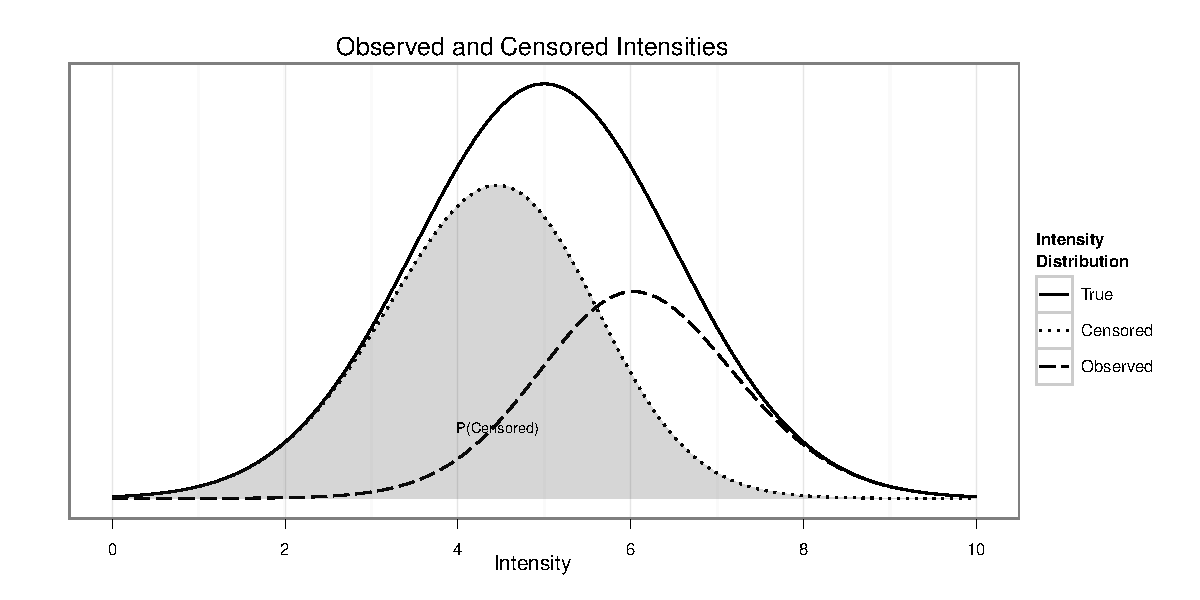
\includegraphics[width=0.8\textwidth]{figures/proteomics/Fig2_Observed_Censored_Intensity_Distributions}
\caption{Comparisons of original, censored, and observed intensity distributions. \label{proteomics:fig:Laplace_Halleys_Outline}}
\end{figure}
\fi

\begin{algorithm}[H]
\caption{$s_{ik}$ Rejection Sampler\label{proteomics:alg:N-Censored-Rejection-Sampler-Algorithm}}

\begin{enumerate}
\item Draw $X\sim NegativeBinomial(1-\hat{p}_{ik}^{*},s_{ik}^{obs}+r)$, with $\hat{p}_{ik}^{*}=(1-\lambda)\left[\pi^{rnd}+(1-\pi^{rnd})\hat{\pi}_{ik}^{IC}\right]$
and $U\sim Uniform(0,1)$.
\item Accept $s_{ik}^{mis}=X$, if $U\leq\begin{cases}
\frac{(s_{ik}^{obs}+s_{ik}^{mis})}{(s_{ik}^{obs}+s_{ik}^{mis}+r-1)} & \text{if }r\geq1\\
\frac{(s_{ik}^{obs}+s_{ik}^{mis})}{s_{ik}^{obs}+s_{ik}^{mis}+r-1}\times\frac{s_{ik}^{obs}+r-1}{s_{ik}^{obs}} & \text{if }0<r<1
\end{cases}$.
\item Return to $1$ otherwise.\end{enumerate}
\end{algorithm}

\ifx\nofigures\undefined
\begin{figure}
\begin{center}
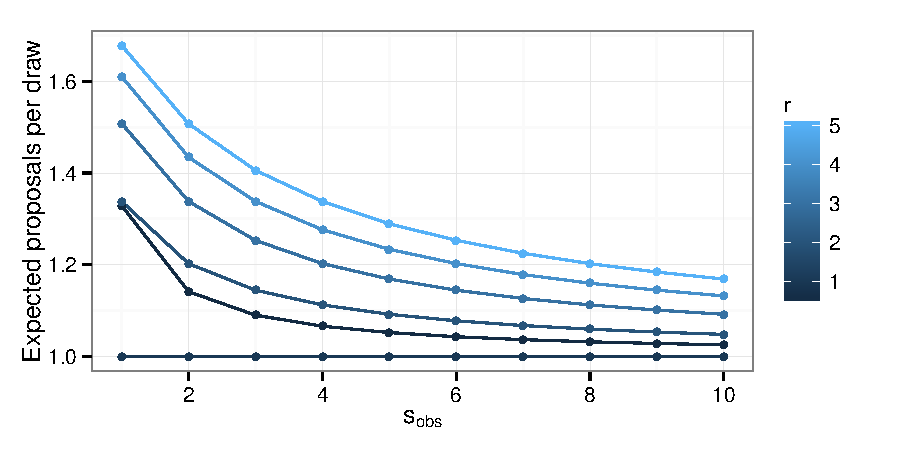
\includegraphics[width=.75\textwidth]{figures/proteomics/figure_nstates_sampler}
\end{center}
\caption{Expected iterations per accepted draw for $s_{ik}^{mis}$ rejection sampler for $\lambda=0.1$, $\pi^{rnd}=0.1$, and $\pi_{ik}^{IC}=.5$, with $r$ ranging from 0.5 to 5, $s_{ik}^{obs}$ ranging from 1 to 10. \label{proteomics:fig:s_ik^mis-Rejection-Sampler}}
\end{figure}
\fi

\subsubsection{Drawing from $p(\bm{R} \mid \bm s, \bm{Y}^{obs}, \bm{\Theta})$} \label{proteomics:sec:r_ik_mis_post}

After drawing the number of states per peptide $s_ik$, we draw the latent random censoring indicators for each censored peptide, $R_{ikl}^{mis}$.
Because random censoring occurs before intensity-based censoring, if a peptide was randomly censored ($R_{ikl}=0$), then $p(I_{ikl}=1\vert R_{ikl}=0,\bm{\Theta})=0$ and $p(O_{ikl}=1\vert R_{ikl}=0,\bm{\Theta})=0$ as outlined in Figure \ref{proteomics:fig:Missing_Data_Indicators_Tree}.
We then obtain the posterior probability that a peptide is randomly censored given that it is missing via a straightforward application of Bayes Theorem:
\begin{eqnarray}
p(R_{ikl}=1\vert O_{ikl}=0,\bm{\Theta}, \bm{Y}^{obs}) & = & 1 - \frac{p(O_{ikl}=0\vert R_{ikl}=0,\bm{\Theta}, \bm{Y}^{obs})p(R_{ikl}=0\vert\bm{\Theta}, \bm{Y}^{obs})}{\sum_{r_{ikl}=0}^{1}p(O_{ikl}=0\vert R_{ikl}=r_{ikl},\bm{\Theta})p(R_{ikl}=r_{ikl}\vert\bm{\Theta}, \bm{Y}^{obs})}\nonumber \\
% & = & \frac{1\times\pi^{rnd}}{\pi^{rnd}\times1+(1-\pi^{rnd})p(O_{ikl}=0\vert R_{ikl}=0,\bm{\Theta})}\label{proteomics:eq:w-posterior-in-text-1}\\
% & = & \frac{\pi^{rnd}}{\pi^{rnd}+(1-\pi^{rnd})\int_{-\infty}^{\infty}p(I_{ikl}=1\vert y_{ikl},R_{ikl}=0,\bm{\Theta})p(y_{ikl}\vert R_{ikl}=0,\bm{\Theta})dY_{ikl}} \label{proteomics:r-posterior}\\
 & = & 1 - \frac{\pi^{rnd}}{\pi^{rnd}+(1-\pi^{rnd})\pi_{ik}^{int}},
\end{eqnarray}
where $\pi_{ikl}^{int}$ is defined as in (\ref{proteomics:eqn:pi_IC}).
Plugging in our numerical approximation for $\pi_{ikl}^{int}$, $\hat{\pi}_{ikl}^{int}$, we draw
\begin{equation}
R_{ikl} \mid \bm{Y}^{obs}, \bm{\Theta}, s_{ik} \sim Bernoulli\left(1 - \frac{\pi^{rnd}}{\pi^{rnd}+(1-\pi^{rnd})\hat{\pi}_{ik}^{int}}\right) .
\end{equation}


\subsubsection{Drawing from $p(\bm{Y}^{mis} \mid \bm{R}, \bm{s}, \bm{Y}^{obs}, \bm{\Theta})$}
\label{proteomics:sec:y_ikl_mis_draw}

The final step in drawing the missing data is to impute the unobserved intensities by drawing each intensity from its full conditional posterior distribution.
The full conditional posterior is given by
\begin{eqnarray*}
p(y_{ikl}^{mis}\vert s_{ik}, R_{ik},\bm{\Theta}) & \propto & \begin{cases}
\phi\left(\frac{y_{ikl} - \gamma_{ik}}{\sigma_{i}}\right) & \text{if }R_{ikl}=0 \text{ and }O_{ikl}=0\\
\phi\left(\frac{y_{ikl} - \gamma_{ik}}{\sigma_{i}}\right) g(y_{ikl}, \bm \eta) & \text{if }R_{ikl}=1 \text{ and }O_{ikl}=0
\end{cases} .
\end{eqnarray*}
For randomly censored states, where $R_{ikl}=0$, the missingness mechanism is ignorable given $R_{ikl}$.
Hence, we simply draw $y_{ikl}^{mis}$ from its unconditional distribution,
\begin{eqnarray*}
p(y_{ikl}^{mis}\vert s_{ik}, I_{ik}=0, R_{ikl}=0, \bm{\Theta}) & \sim & Normal(\gamma_{ik},\sigma_{i}^{2}).
\end{eqnarray*}
%
The posterior distribution for intensity-censored states ($R_{ikl}=1$, $I_{ikl}=0$) is given by
\begin{eqnarray}
p(y_{ikl}^{mis}\vert O_{ikl}=0,R_{ikl}=1,\bm{\Theta}) & = & (\pi_{ik}^{int})^{-1}\frac{1}{\sigma_{i}} \phi\left(\frac{y_{ikl}^{mis}-\gamma_{ik}}{\sigma_{i}}\right) g(y_{ikl}^{mis}, \bm \eta) .
\label{proteomics:eq:intensity-censored-posterior-text}
\end{eqnarray}
As this is not a standard distribution, we draw from it using a rejection sampler.
We use information from the adaptive quadrature of Section \ref{proteomics:sc:draw_s_ik_mis} to construct an efficient proposal distribution with little additional computation.
Specifically, we propose from a location-scale transformation of a $t_{\nu}$-distribution as
\begin{eqnarray}
Y_{ikl}^{*} & \sim & \hat{y}_{ikl}^{mis}+\hat{\sigma}_{ik}^{mis} \sqrt{\frac{\nu-2}{\nu}} t_{\nu},
\end{eqnarray}
which has expectation $\hat{y}_{ik}^{mis}$ and variance $\hat{\sigma}_{ik}^{mis})^{2}$ for $\nu>2$.

The rejection sampling algorithm requires bounding the ratio of the target density to the proposal density.
For this sampler, the given ratio has two local maxima, as shown in Figure \ref{proteomics:fig:Censored-Intensity-Rejection-Sampler-Outline-TEXT} B and C.
The global maximum of the ratio can be either the first or third root of the log-ratio's derivative depending upon the particular relationship between $\bm \eta$, $\sigma^2_i$, and $\gamma_ik$.
To reliably find the global maximum of the target-proposal density ratio, we use a pair of vectorized bisection searches to find the roots of the derivative of the log-ratio in two ranges: $(-\infty,\hat{y}_{ik}^{mis})$ and $(\hat{y}_{ik}^{mis},\infty)$.
Once these roots are obtained, we simply select the one corresponding to the larger local maximum to compute acceptance probabilities.
A graphical example of the rejection sampler is shown in Figure \ref{proteomics:fig:Censored-Intensity-Rejection-Sampler-Outline-TEXT} D, and the sampling algorithm is detailed in Algorithm \ref{proteomics:alg:Censored-Intensity-Accept-Reject-Algorithm-TEXT}.

\ifx\nofigures\undefined
\begin{figure}
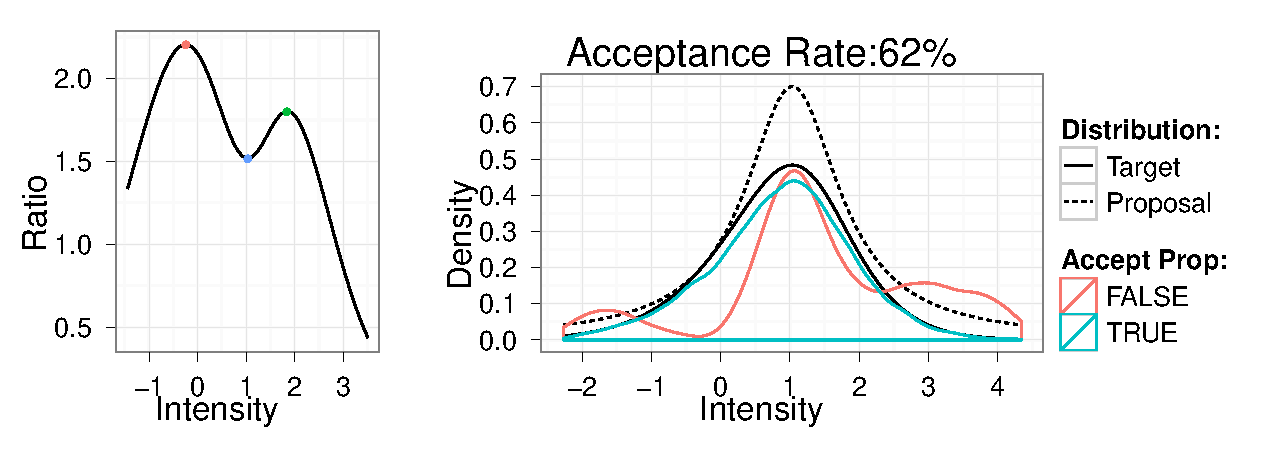
\includegraphics[width=1\textwidth]{figures/proteomics/figure_ycen_rejection_sampler.pdf}
\caption{Censored Intensity Rejection Sampler Example\label{proteomics:fig:Censored-Intensity-Rejection-Sampler-Outline-TEXT}}
\end{figure}
\fi

\begin{algorithm}
\caption{$y_{ikl}^{mis}$ rejection sampler algorithm\label{proteomics:alg:Censored-Intensity-Accept-Reject-Algorithm-TEXT}}


$ $Target density: $f^{mis}(y_{ikl}\vert\eta_{0},\eta_{1},\gamma_{ik},\sigma_{i}^{2})=(\pi_{ik}^{int})^{-1} \frac{1}{\sigma_{i}}\phi\left(\frac{y_{ikl}-\gamma_{ik}}{\sigma_{i}}\right) g(y_{ikl}, \bm \eta)$.

Proposal density: $f^*(y_{ikl}^{*}\vert\nu,\tilde{\mu}_{ikl},\tilde{\sigma}_{ikl})=\frac{\Gamma\left(\frac{\nu+1}{2}\right)}{\sqrt{\nu\pi}\Gamma\left(\frac{\nu}{2}\right)}\left(1+\frac{(y_{ikl}^{*}-\tilde{\mu}_{ikl})^{2}}{\nu\tilde{\sigma}_{ikl}^{2}}\right)^{-\left(\frac{\nu+1}{2}\right)}$.
\begin{enumerate}
\item Compute $z_{ikl}$:

\begin{enumerate}
\item Using bisection, find the roots of of the first derivative of the
log density ratio, \\
$z_{ikl}^{(1)}\equiv\underset{y_{ikl}\in[-\infty,\tilde{\mu}_{ikl})}{\arg\max}\log\left[\frac{f^{mis}(y_{ikl}\vert\eta_{0},\eta_{1},\gamma_{ik},\sigma_{i}^{2})}{f^*(y_{ikl}\vert\nu,\tilde{\mu}_{ikl},\tilde{\sigma}_{ikl})}\right]$
and $z_{ikl}^{(2)}\equiv\underset{y_{ikl}\in(\tilde{\mu}_{ikl},\infty]}{\arg\max}\log\left[\frac{f^{mis}(y_{ikl}\vert\eta_{0},\eta_{1},\gamma_{ik},\sigma_{i}^{2})}{f^*(y_{ikl}\vert\nu,\tilde{\mu}_{ikl},\tilde{\sigma}_{ikl})}\right]$.
\item Determine the maximum of the density ratios,\\
 $c^* \equiv \max\left(\frac{f^{mis}(z_{ikl}^{(1)}\vert\eta_{0},\eta_{int},\gamma_{ik},\sigma_{i}^{2})}{f^*(z_{ikl}^{(1)}\vert\nu,\tilde{\mu}_{ikl},\tilde{\sigma}_{ikl})},\frac{f^{mis}(z_{ikl}^{(2)}\vert\eta_{0},\eta_{1},\gamma_{ik},\sigma_{i}^{2})}{f^*(z_{ikl}^{(2)}\vert\nu,\tilde{\mu}_{ikl},\tilde{\sigma}_{ikl})}\right)$.
\end{enumerate}
\item Generate $X\sim g(y_{ikl}^{*}\vert\nu,\tilde{\mu}_{ikl},\tilde{\sigma}_{ikl})$,
$U\sim Unif(0,1)$.
\item Accept $y_{ikl}=X$, if $U\leq\frac{f^{mis}(X\vert\eta_{0},\eta_{int},\gamma_{ik},\sigma_{i}^{2})}{c^* f^*(X\vert\nu,\tilde{\mu}_{ikl},\tilde{\sigma}_{ikl})}$.
\item Else, return to $2$.\end{enumerate}
\end{algorithm}


 %%% %%% %%%
 %%% %%% %%%


\section{Simulation studies}
\label{proteomics:sec:simulations}

To evaluate the performance of our method and the stability of the algorithm presented in Section \ref{proteomics:sec:estimation}, we tested our method on a set of simulated MS-MS experiments.
We describe the design of these simulations in detail in Section \ref{proteomics:sec:doe}.
We cover the computational performance and validation of our MCMC sampler in Section \ref{proteomics:sec:mcmc_performance}.
In Section \ref{proteomics:sec:frequentist_evaluations}, we evaluate the frequentist properties of our Bayesian estimates, including the coverage of our posterior intervals (\ref{proteomics:sec:coverage}) and the performance of the proposed method relative to standard estimators used for this class of experiments (\ref{proteomics:sec:compperf}).

 %%% %%% %%%
 %%% %%% %%%
 %%% %%% %%%

\subsection{Design of experiments}
\label{proteomics:sec:doe}

We simulated a set of complex biological samples, spanning a broad range of abundances and protein-specific properties.
For each such sample we simulate 54 proteins with abundances spanning 6 orders magnitude, $\mu_i= 3, \ldots, 8$, yielding 9 proteins per abundance level.
Within each abundance level, each simulated protein consists of $m_{ik}=20,25\ldots,60$ peptides.
With these properties fixed across replicates, we simulated 1,200 experiments from the model described in Section \ref{proteomics:sec:model}, using a probit link function for $g(\cdot, \bm \eta)$.
These consisted for 400 replicates for each of the parameter settings provided in Table \ref{proteomics:table:sim_parameters}, each of which was based on estimates from an experiment with the given gradient length using the Sigma UPS2 standard.

\ifx\nofigures\undefined
\begin{table}
\begin{center}
\caption{Parameter settings for simulation studies.
\label{proteomics:table:sim_parameters}}
\begin{tabular}{r|ccccccccc}
  \hline
Gradient & $\alpha_\tau$ & $\beta_\tau$ & $\alpha_\sigma$ & $\beta_\sigma$ & $\pi^{rnd}$ & $\eta_0$ & $\eta_1$ & $\lambda$ & $r$ \\ 
  \hline
   90m & 6.3 & 2.1 & 8.5 & 3.5 & 0.20 & 16 & -3.0 & 0.84 & 1.9 \\ 
  180m & 5.3 & 1.3 & 7.0 & 4.1 & 0.21 & 14 & -2.7 & 0.79 & 1.9 \\ 
  360m & 6.2 & 1.8 & 7.0 & 2.5 & 0.30 & 20 & -4.3 & 0.62 & 1.6 \\ 
   \hline
\end{tabular}
\end{center}
\end{table}
\fi

%Across these experiments, we fixed our top-level parameters to the following values: $\alpha_\tau=4$, $\beta_\tau=5$, $\alpha_\sigma=8$, $\beta_\sigma=4$, $\pi^{rnd}=0.1$, $\eta_0=-6.25$, $\eta_1=1.25$, $\lambda=0.1$, and $r=3$.


%% why these values? add a paragraph with some comments on the values; what observable properties they imply (e.g., 50% missing at .. and 10% missing at ..). how many state-level intensities (data points) on average in each data set?
%These values were selected based upon initial estimates from experiments using the Sigma UPS2 standard.
%They imply 50\% missingness at an intensity of $5.18$, 90\% missingness at an intensity of 3.34, and 15\% missingness at an intensity of 7.27.
%These also imply a mean of $1.33$ possible states per peptide with 99\% having between 1 and 4 possible states.
%The variance parameters yield $E[\sigma_i] = 1.39$ and $E[\tau_i] = 0.87$, with 95\% of their values within $(0.93, 1.90)$ and $(0.47, 1.32)$, respectively.
%These reflect a typical regime for both the missingness mechanism and the degree of variation observed in MS-MS data.


\subsection{MCMC performance and validation}
\label{proteomics:sec:mcmc_performance}

Our MCMC sampler produced high-quality draws from the target posterior at a low computational cost.
Running 3,000 iterations for each replicate required an average of 267 seconds (0.088 seconds per iteration) with a standard deviation of 17.1 seconds.
Of these 3,000 iterations, we discarded the first 1,000 as burn in.
The mean effective sample sizes for each top-level parameter based on the remaining 2,000 draws are provided in Table \ref{proteomics:tab:effective_sample_sizes}.
For $\mu_i$ and $\zeta_i$, we also include the mean standard deviation of effective sample sizes across proteins.
%
\ifx\nofigures\undefined
\begin{table}
\centering
\caption{Average effective sample sizes by parameter. $\pm$ for $\mu_{i}$
and $\zeta_{i}$ indicates the average standard deviation of effective
sample sizes across proteins. \label{proteomics:tab:effective_sample_sizes}}
\begin{tabular}{r|cccccccccc}
\hline 
Gradient  & $\zeta_{i}$ & $\eta$  & $\lambda$ & $\mu_i$  & $\pi^{rnd}$ & $r$ & $\beta_{\sigma}$ & $\beta_{\tau}$ & $\alpha_{\sigma}$ & $\alpha_{\tau}$\tabularnewline
\hline 
90m  & 341$\pm$188  & 287  & 773  & 331$\pm$191 & 191  & 1160  & 272  & 217  & 303  & 242 \tabularnewline
180m  & 256$\pm$143 & 285  & 823  & 250$\pm$148 & 175  & 1197  & 337  & 176  & 379  & 191 \tabularnewline
360m  & 421$\pm$208 & 179  & 1013  & 411 $\pm$215 & 275  & 1338  & 346  & 222  & 392  & 250 \tabularnewline
\hline 
\end{tabular}
\end{table}
\fi
%
We note that all mean effective sample sizes are greater than 100, indicating that even 2,000 iterations are sufficient to obtain Monte Carlo  an order of magnitude below the posterior standard deviation of each parameter.

\subsection{Frequentist evaluations}
\label{proteomics:sec:frequentist_evaluations}

\subsubsection{Coverage analysis}
\label{proteomics:sec:coverage}

We first used our simulated replicates to evaluate the frequency coverage of our posterior intervals, focusing on those for $\zeta_i$.
The results of these evaluations are summarized in Figure \ref{proteomics:fig:coverage_mu_hpd}; corresponding results for coverage vs. $m_i$ are similar and provided in Appendix \ref{ch:supp:proteomics}.
%
\ifx\nofigures\undefined
\begin{figure}
\centering
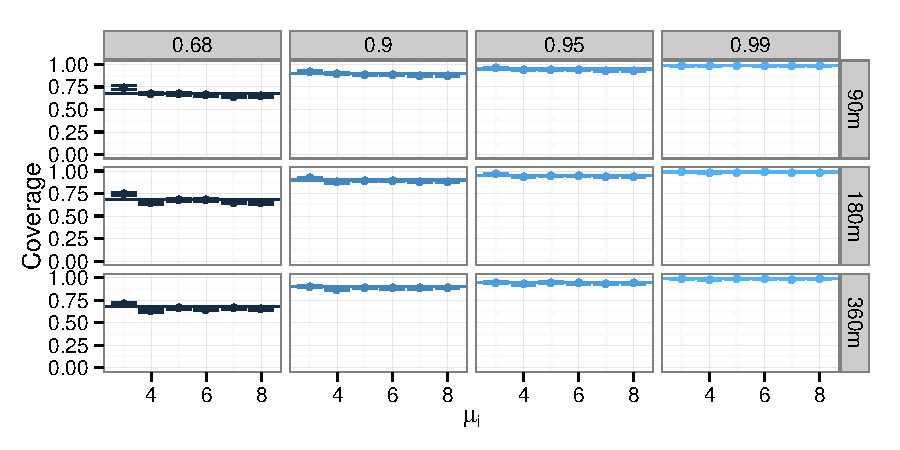
\includegraphics[width=\textwidth, page=1]{figures/proteomics/figures_coverage_sim}
\caption{Coverage of HPD intervals vs. $\mu_i$ by simulated gradient length and Bayesian level.
\label{proteomics:fig:coverage_mu_hpd}}
\end{figure}
\fi
%
We find that our posterior intervals are well-calibrated for the regimes of interest.
Across all three simulated gradient lengths, we obtain 67\% coverage for our 68\% posterior intervals, 89\% mean coverage for our 90\% posterior intervals, 94\% mean coverage for our 95\% posterior intervals, and 98\% mean coverage for our 99\% posterior intervals.
These demonstrate that, despite the complexity of our Bayesian method, it can provide inferences with frequentist guarantees.

%\ifx\nofigures\undefined
%\begin{figure}
%\centering
%\includegraphics[width=\textwidth, page=3]{figures/proteomics/figures_coverage_sim}
%\caption{Coverage of HPD intervals vs. $m_i$ by simulated gradient length and Bayesian level.
%\label{proteomics:fig:coverage_mi_hpd}}
%\end{figure}
%\fi

\subsubsection{Comparison with exiting methods}
\label{proteomics:sec:compperf}

We compared the performance of our model-based abundance estimates with several standard methods for absolute protein quantitation.
Many of these methods were originally developed for relative quantitation and are converted to absolute measures by appropriate rescaling.
All methods used in this comparison are of the form
\begin{equation}
 \hat{\zeta}_i = \log_{10}\left( \hat{T} \frac{10^{\hat{\mu}_i}}{\sum_i 10^{\hat{\mu}_i}} \right) .
\end{equation}
%
We compare the performance of our method to two classes of common methods: intensity-based estimators and count-based estimators.
We set $\hat{T} = \sum_i 10^{\mu_i}$ for all of these estimators.
Among intensity-based estimators, we consider simple summed intensities  (\ref{proteomics:eq:summed_intensity}) and median observed intensity  (\ref{proteomics:eq:median_intensity}) \citep[e.g.,][]{Cox:2008uu}.
We also evaluate two variants based on estimators from the spectral counting literature: mean observed intensity (\ref{proteomics:eq:mean_intensity}) and adjusted mean observed intensity (\ref{proteomics:eq:adj_mean_obs_intensity})
\begin{eqnarray}
\hat \mu_{i}^{si} &=& \log_{10} \left( \sum_{kl} 10^{y^{obs}_{ikl}} \right),
\label{proteomics:eq:summed_intensity} \\
\hat \mu_{i}^{med} &=& \text{Med}_{kl}(y_{ikl}),
\label{proteomics:eq:median_intensity} \\
\hat \mu_{i}^{mi} &=& \log_{10}\left( \sum_{kl} 10^{y^{obs}_{ikl}}/m_i^{obs} \right),
\label{proteomics:eq:mean_intensity} \\
\hat \mu_{i}^{ami} &=& \log_{10}\left( \sum_{kl} 10^{y^{obs}_{ikl}}/\sum_{k} s^{obs}_{ik} \right) .
\label{proteomics:eq:adj_mean_obs_intensity}
\end{eqnarray}
%
In the above, $m_i$ is the (known) number of possible peptides that are generated by digesting protein $i$ using a particular enzyme.

Another common approach, known as spectral counting, disregards the intensity measurements and uses counts of the observed states associated with each protein.
A range of such methods have been developed relative quantitation, including basic spectral counting \citep[e.g.,][]{Liu:2004hv}, average spectral counts \citep[e.g.,][]{Weiss:2010ik}, and the proportion of peptides identified (PPI) \citep{Rappsilber2002}.
However, these are not directly suitable for absolute quantitation due to a lack of normalization.
\citet{Ishihama:2005ir} defined an exponentially-modified protein abundance index (emPAI) to address these issues:
%
\begin{equation}
\hat \mu_{i}^{emPAI} = \log_{10}\left( 10^{\sum_k \mathbb{I}(s_{ik}^{obs} > 0) / m_i } - 1 \right) .
\label{proteomics:eq:empai}
\end{equation}
This provides a commonly-used representative of the count-based class of methods.

We summarize the results of these comparisons in Figures \ref{proteomics:fig:compare_relative_error} and \ref{proteomics:fig:compare_bias}.
%
\ifx\nofigures\undefined
\begin{figure}
\centering
\includegraphics[width=\textwidth, page=3]{figures/proteomics/figures_relative_error_sim}
\caption{Relative efficiency of standard methods ($MSE_{Method} / MSE_{Model-based}$) vs. $\mu_i$ and $m_i$ by block (left and right columns, respectively). Relative MSE axis is logarithmic. Solid black line at 1 corresponds to the model-based method's efficiency, by definition.
\label{proteomics:fig:compare_relative_error}}
\end{figure}
\fi
%
Complete tabular results are available in Appendix \ref{ch:supp:proteomics}.
From Figure \ref{proteomics:fig:compare_relative_error}, we see that our method reduces the overall MSE of abundance estimates by a factor of 5--10 relative to intensity-based estimates and by a factor of 6--150 relative to emPAI.
Most intensity-based estimators exhibit consistent efficiency relative to ours, although the median intensity estimator's efficiency improves to nearly 1 as abundance increases.
However, this estimator's efficiency is quite poor for low-abundance proteins with approximately 20 times the model-based estimator's MSE.
The efficiency of emPAI increases by an order of magnitude over the range of simulated abundances and decreases slightly with protein length $m_i$, demonstrating the value of intensity information in low-abundance regimes.
By carefully combining count and intensity information, we obtain consistent reductions in MSE relative to both classes of methods for all values of $\mu_i$ and $m_i$.

\ifx\nofigures\undefined
\begin{figure}
\centering
\includegraphics[width=\textwidth, page=3]{figures/proteomics/figures_bias_sim}
\caption{Bias of $\hat{\zeta}_i$ for standard methods and posterior mean from model vs. $\mu_i$ and $m_i$ by gradient length (left and right columns, respectively).
\label{proteomics:fig:compare_bias}}
\end{figure}
\fi
%
Turning to bias, we see that the model-based estimator provides lower bias than both classes of standard methods.
Summed intensity shows a slight negative bias (between -0.7 and 0), while mean and average mean observed intensity show a positive bias of similar magnitude.
The median intensity estimator shows a far larger positive bias (nearly 2 orders of magnitude) at low abundances.
The biases of all four intensity-based estimators diminish as abundance increases.
The emPAI estimator shows a large positive bias that also decreases in magnitude with abundance.
The bias of the summed intensity estimator diminishes from approximately -0.7 to 0 as protein length increases; the biases of our other estimators exhibits little sensitivity to protein length.
Again, we see that our model-based approach enables us to combine count and intensity information into estimators that outperform both classes of standard methods.

 %%% %%% %%%
 %%% %%% %%%


\section{Empirical results}
\label{proteomics:sec:empirical}

Having established our method's properties on simulated data, we turn to actual experimental data.
We use a quantitative protein standard, described in Section \ref{proteomics:sec:data}, for these experiments.
This standard provides known abundances for evaluation with a realistic set of proteins.
In Section \ref{proteomics:sec:checkassumptions}, we use these experiments to check our model assumptions and demonstrate their implications for real data.
In Section \ref{proteomics:sec:dataanalysis}, we assess the comparative performance of the proposed methods with respect to the standard methods presented in Section \ref{proteomics:sec:compperf}.

 %%% %%% %%%
 %%% %%% %%%

\subsection{Data}
\label{proteomics:sec:data}

We conducted a set of LC/MS-MS experiments using the Universal Proteome Standard 2 (UPS2), a constructed biological sample that contains 48 human proteins.
These proteins are present in six concentrations, ranging from .5fM to 50,000 fM, with eight known proteins at each concentration.
These proteins are selected to span a broad range of physical properties (size and hydrophobicity) within each concentration, removing a potential confounding factor while reflecting the actual variation among proteins in typical samples.
The concentration specified for each protein in the standard was confirmed by the manufacturer using multiple methods, so we are comfortable taking the concentrations reported by the manufacturer as ground truth for subsequent analyses.
With its high dynamic range, the standard provides a realistic and stringent test of our method.

We ran five LC/MS-MS experiments using this standard at three gradient lengths, 90, 180, and 360 minutes, with two, two, and one replicates per gradient length, respectively.
Each gradient length implies a different set of parameters for the missing data mechanism.
Longer gradients allow for the observation of a greater variety MS2 spectra and is expected to decrease the degree of intensity-based missingness.
However, longer gradients can also reduce the dynamic range of observed intensities and require substantially greater effort from the experimenter.
Our experiments allow us to explore these tradeoffs in as we evaluate our method.
The 90 minute gradients reflect the degree of censoring typically observed in analyses of more complex mixtures, while the 180 and 360 minute gradients provide a ``sanity check'' of our method's behavior in a setting with less missing data.

 %%% %%% %%%
 %%% %%% %%%

\subsection{Exploratory analysis and model checking}
\label{proteomics:sec:checkassumptions}

Using the experimental data, we examined the distributions of intensities, identifications, and states to check the assumptions of our model.
Figure \ref{proteomics:fig:EDA-Figure} summarizes these results.
%
\ifx\nofigures\undefined
\begin{figure}
\centering
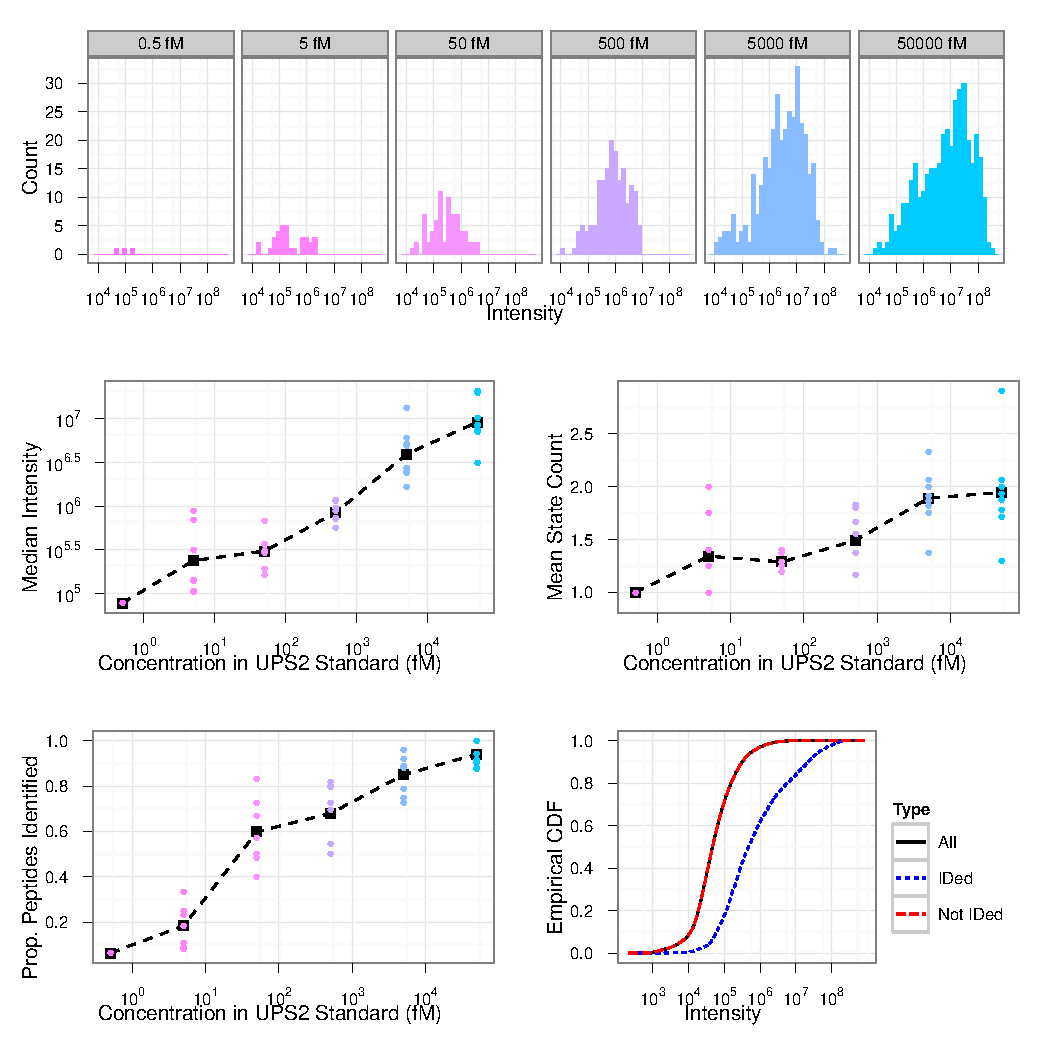
\includegraphics[width=\textwidth]{figures/proteomics/New_EDA_Multipanel_Figure}
\caption{Exploratory data analysis using the UPS2 quantitative protein standard.
\label{proteomics:fig:EDA-Figure}}
\end{figure}
\fi
%
Panel A of this figure shows the observed distribution of intensities by concentration.
It is immediately clear from these histograms that the number of intensities observed and the median observed intensity increases strongly with the concentration.
The distributions of observed intensities are also right-skewed for each concentration level, which is consistent with the combination of intensity-dependent censoring and an underlying log-normal distribution of intensities.

Panels B, C, and D show the relationship between concentration and identification, median intensity, and $s_{ik}^{obs}$ in greater detail.
The median observed intensity by protein increases with the protein's concentration, although the former has far less dynamic range than the latter (2 orders of magnitude vs. 5).
Intensity-based censoring at the state level explains this discrepancy, as the lowest-intensity ions are preferentially removed from the sample.
%
We also compared the number of states that peptides were detected in across protein concentrations.
The physical process that generates distinct peptide states is known to be independent of protein or peptide abundance, so the number of \emph{possible} peptide states must be invariant to the peptide's concentration.
Since it is not possible to determine the number of possible states per for peptide \emph{a priori}, we model this value as an IID random variable in our model.
However, we observe a strong relationship between the number of observed peptide states and concentration in the experimental data.
This supports the assumption of intensity-dependent state-level censoring in our model.

The proportion of peptides identified per protein ranges nearly 1 for the most abundant proteins to approximately 5\% for the least abundant, while the 
This is mostly attributable to selection for abundant ions within the MS-MS equipment, as panel E demonstrates.
By design, the subset of peptides selected for fragmentation is determined by the instrument's software in real time as the sample is analyzed.
While we focus on the subset of peptides that are both detected by the mass spectrometer and successfully identified, nearly all of the peptides in the sample can be quantified in terms of their total intensity\footnote{
Software is able to quantify peptides that were not identified is due to the both mass accuracy of the mass spectrometer and the effective separation of the sample by chromatography.
The software used to process the experimental data \citep{Cox:2008uu} is able to identify and integrate over all unique profiles in the m/z $\times$ intensity $\times$ retention time space, as shown in Figure \ref{proteomics:fig:Mass_Spec_Overview} C.
This allows quantitation of the majority of peptides; however, since the majority of these are not identified, there is no way to map them to a specific protein.
Hence, we exclude them from our model-based inference.}.
This allows us to investigate the intensity-dependence of the peptide identification process in detail and validate our model assumptions.
Comparing the distributions of identified and unidentified state-level intensities in Panel E shows that (1) the distribution of identified intensities stochastically dominates that of the unidentified intensities and (2) there is substantial overlap between these distributions.
(1) is consistent with Theorem \ref{proteomics:thm:dominance}, while (2) is consistent with the assumption of a stochastic censoring mechanism.

 %%% %%% %%%
 %%% %%% %%%

\subsection{Comparison of empirical results}
\label{proteomics:sec:dataanalysis}

We used the experiments described in Section \ref{proteomics:sec:data} to evaluate our method's performance against the standard methods described in Section \ref{proteomics:sec:compperf}.
We summarize these results in Figure \ref{proteomics:fig:UPS2 results} and Table \ref{proteomics:tab:UPS2 results} and provide complete tables of results in Appendix \ref{ch:supp:proteomics}.
%
\ifx\nofigures\undefined
\begin{figure}
\centering
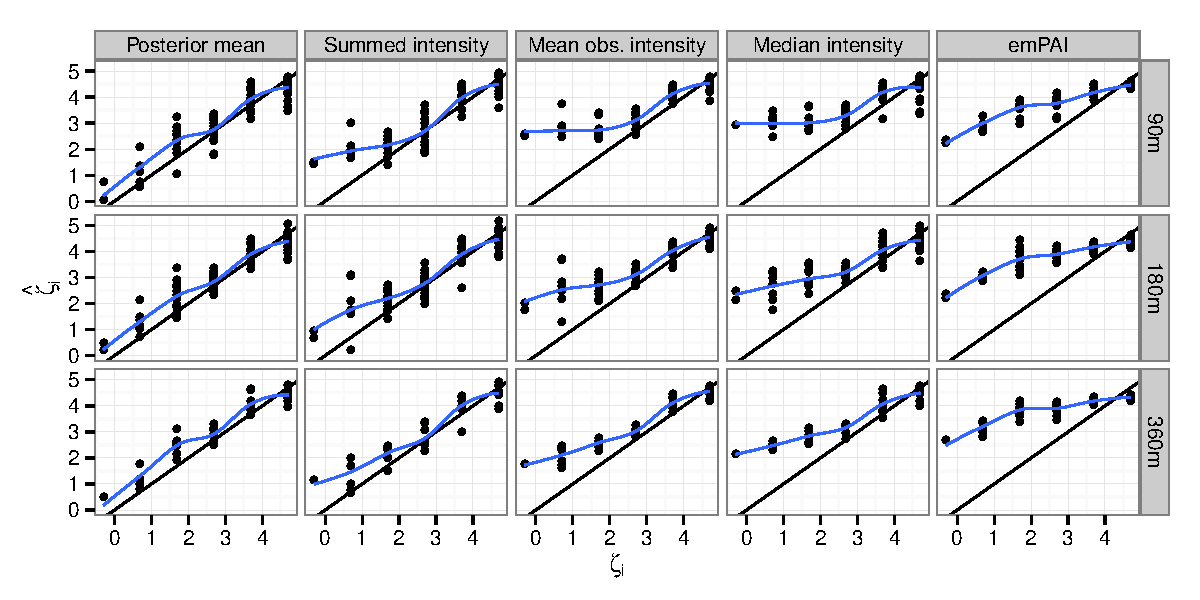
\includegraphics[width=\textwidth]{figures/proteomics/figures_draft_ups2}
\caption{Inferred protein abundances from experiments with UPS2 standard.
\label{proteomics:fig:UPS2 results}}
\end{figure}
\fi
%
\ifx\nofigures\undefined
\begin{table}
\centering
\caption{Mean squared errors $\pm$ standard errors from experiments with UPS2 standard.
\label{proteomics:tab:UPS2 results}}
%\begin{tabular}{l|ccccc}
%  \hline
%Gradient & Posterior mean & Summed intensity & Mean obs. intensity & Median intensity & emPAI \\ 
%  \hline
%90m & $0.41 \pm 0.11$ & $1.06 \pm 0.12$ & $2.45 \pm 0.16$ & $3.18 \pm 0.13$ & $2.81 \pm 0.10$ \\ 
%  180m & $0.34 \pm 0.07$ & $0.76 \pm 0.14$ & $1.82 \pm 0.21$ & $2.26 \pm 0.21$ & $3.03 \pm 0.12$ \\ 
%  360m & $0.37 \pm 0.06$ & $0.65 \pm 0.07$ & $1.26 \pm 0.08$ & $1.87 \pm 0.06$ & $3.55 \pm 0.13$ \\ 
%   \hline
%\end{tabular}
\begin{tabular}{l|ccc}
\hline
& \multicolumn{3}{c}{Gradient length} \\
  \hline
Method & 90m & 180m & 360m \\ 
  \hline
Posterior mean & $0.41 \pm 0.11$ & $0.34 \pm 0.07$ & $0.37 \pm 0.06$ \\ 
  Summed intensity & $1.06 \pm 0.12$ & $0.76 \pm 0.14$ & $0.65 \pm 0.07$ \\ 
  Mean obs. intensity & $2.45 \pm 0.16$ & $1.82 \pm 0.21$ & $1.26 \pm 0.08$ \\ 
  Median intensity & $3.18 \pm 0.13$ & $2.26 \pm 0.21$ & $1.87 \pm 0.06$ \\ 
  emPAI & $2.81 \pm 0.10$ & $3.03 \pm 0.12$ & $3.55 \pm 0.13$ \\ 
   \hline
\end{tabular}
\end{table}
\fi
%
We restrict our attention here to the best-performing subset of the estimators presented in Section \ref{proteomics:sec:compperf}.
We see from Table \ref{proteomics:tab:UPS2 results} that our method's performance is particularly strong on short gradients, providing a factor of 2.6 reduction in MSE relative to the best standard estimator (summed intensity) for the 90 minute gradients and a factor of 2.2 reduction for the 180 minute gradients.
On the longest gradient (360 minutes), our method's MSE is a factor of 1.8 lower than than that of the best standard estimator.
This behavior matches our expectations based on the relevant properties of the underlying experimental processes.
Detailed modeling of the missing data mechanism yields the largest gains when the sample is least separated and there are fewer possible spectra---in the shortest gradients.
In the longest gradient, intensity-based missingness diminishes in importance relative to other factors.

From Figure \ref{proteomics:fig:UPS2 results}, we note that our method's improvements are greatest for low-abundance proteins.
All estimators considered provide reasonably good estimates of $\zeta_i$ for the highest-abundance proteins.
However, most of the standard estimators exhibit a substantial positive bias (1-2 orders of magnitude) for the lowest-abundance proteins, particularly on short gradients.
In contrast, our method provides consistently accurate estimates for low-abundance proteins across all gradient lengths.
We discuss the implications of this capability for biological applications in Section \ref{proteomics:sec:remarks}.
%However, the mean intensity estimator appears to perform better on this measure.
%This estimator implicitly imputes zeros for all unobserved peptide intensities by using the number of predicted peptides $m_i$ as a denominator, correcting for some of the positive bias in observed intensities.
%This implicit correction is not sufficient to yield accurate results on the shorter gradients, though.



 %%% %%% %%%
 %%% %%% %%%

\section{Concluding remarks}
\label{proteomics:sec:remarks}

We have presented a model-based approach to label-free absolute quantitation in LC/MS-MS proteomics experiments.
As the results of Sections \ref{proteomics:sec:simulations} and \ref{proteomics:sec:empirical} show, accounting for non-ignorable missing data in the proteomics context improves estimates of absolute abundances.
Our method also provides well-calibrated measures of uncertainty, as the results of Sections \ref{proteomics:sec:coverage} and \ref{proteomics:sec:dataanalysis} show.
Below, we provide some broader context and particular insights on this class of methods and problems, focusing on the role of non-ignorable missing data in complex experiments, efficient computation with missing data of variable dimension, and the role of absolute quantitation in biological analyses.
We also discussion extensions of the methods presented to the semi-supervised setting and distributed computational environments.

\subsection{Modeling and inference}

The core of our model for LC-MS/MS proteomics data is the structure of our non-ignorable missing data mechanism.
We explicitly account for the dependence of censoring probabilities on unobserved peptide intensities at the level of individual peptide states.
This creates an additional complication, as the number of possible states per peptide is unknown.
Thus, we must account for truncation at the state level in addition to censoring at the peptide level.
However, we do know that the distribution of then number possible peptide states is invariant to the peptide's concentration.
Incorporating this information into our model allows us to extract information from the number of states observed per peptide ($s_{ik}^{obs}$).

Working with state-level data provides fine-grained measures of missingness, which provide a great deal of information on low-abundance proteins when used properly.
For high-abundance proteins, the vast majority of peptide states are observed, providing the majority of the information on the underlying distribution of the number of states per peptides.
Our model uses this information to improve inferences on the abundances of low-abundance proteins, leveraging all of the available information from their intensity and state information.
Extracting all of this information requires a sophisticated approach to inference and computation, however.

The presence of state-level censoring with an unknown number of states per peptide makes inference under our missing data model particularly challenging.
The dimension of our missing data $\bm M$ varies across draws, requiring more specialized computational strategies than standard Metropolis-Hastings updates.
We implemented an exact marginal draw from the conditional distribution of $\bm M$ given $\bm \Theta$ using a combination of unidimensional numerical integration and efficient rejection sampling, as detailed in Section \ref{proteomics:sec:missingDataDraw}.
The reductions in autocorrelation provided by this marginal update more than offset the computational costs of rejection sampling and numerical approximation.
This allows for efficient inference in the presence of missing data of unknown dimension, as the results of Section \ref{proteomics:sec:simulations} demonstrate.
We believe that this technique can provide effective computational techniques for a range of non-ignorable missing data problems originating from complex experimental techniques.

\subsection{Applications}

Absolute quantitation provides a different view on biological processes than relative quantitation, enabling the study of new phenomena.
Whereas relative quantitation can only measure the protein-by-protein differences in abundances across experiments, absolute quantitation provides estimates of the abundances of different proteins within a single population of cells.
Such information is somewhat interesting for high-abundance proteins, but it promises the greatest insights from the study of low-abundance ones.

Reliable, accurate quantitation of low-abundance proteins also makes LC/MS-MS methods applicable to new classes of biological investigations.
Two of the most promising areas are the study of mistranslation and transcription factors.
Both involve proteins which appear at low concentrations but can have an outsized biological impact.
In the case of mistranslation, the cell must spend a great deal of energy handling defective proteins; the rate of mistranslation represents the largest determinant of these costs.
Transcription factors regulate the conversion of DNA into mRNA, providing one of the primary mechanisms of control and feedback for cellular functions.
Our method allows for reliable estimates of these proteins' concentrations within large populations of cells, opening new areas for high-throughput research.

\subsection{Extensions}

We are developing two extensions of the proposed methodology with a focus on larger, shallower datasets.
In relatively shallow datasets, few proteins are observed and, due to intensity-based censoring, the dynamic range of observed intensities is compressed.
This makes estimation of the censoring parameters ($\eta$ and $\pi^{rnd}$) from observed data difficult, reducing the precision of our estimates.
The quantitative protein standard described in Section \ref{proteomics:sec:data} provides a potential solution to this problem.
Such a standard can be spiked into the biological sample of interest and used as a calibration source.
A semi-supervised version of the model presented in Section \ref{proteomics:sec:model} can use the known properties of this standard to enable reliable inferences about the censoring mechanism in shallow samples.
As an additional benefit, this supervision could simplify the conversion of our estimates between the intensity and abundance scales.

To tackle larger datasets, including full-proteome quantitation for complex organisms, we are also developing a distributed variant of the MCMC algorithm presented here.
The goal is to scale the sampler across computational clusters with minimal communication within iterations.
The conditional independence structure of the model presented in Section \ref{proteomics:sec:model} makes such distribution both appealing and feasible.

We see a rich range of opportunities for statistical research in this area.
The field of MS-MS proteomics is young, and it can provide a unique view on the details of biological processes.
Extracting this technology's full value requires care, deep subject-matter knowledge, and sophisticated statistical techniques, but the rewards are great.
We hope that more statisticians will enter this field and continue to build strong methodological foundations to advance biological research.

 %%% %%% %%%
 %%% %%% %%%
 %%% %%% %%%

\section{Acknowledgments}

This work was partially supported by the National Science Foundation under grants no.\ DMS-0907009 and no.\ IIS-1017967, by the National Institute of Health under grant no.\ R01 GM-096193, all to Harvard University. Additional funding was provided by the Harvard Medical School's Milton Fund.
%%
%The views and conclusions contained in this document are those of the  authors and should not be interpreted as representing the official policies, either expressed or implied, of the National Institute of Health, the Army Research Office, the National Science Foundation, or the U.S. government.

 %%% %%% %%%
 %%% %%% %%%
 %%% %%% %%%

%\appendix

\section{Proof of Theorem \ref{proteomics:thm:dominance}}
\label{proteomics:sec:proof1}

\begin{proof}
Define $Y$ as a random variable with a distribution given by
%
\begin{equation}
\nonumber
\dd F_Y(y) = \frac{1}{w} g(y) \dd F_x(y)
\end{equation}
%
where $w \equiv \int_{\Reals} g(t) \dd F_x(t) \equiv P(Z=1)$. We assume we are in a non-trivial case, so $w \in (0,1)$.
%
Then, define $h \equiv g^{-1}(w)$. Consider the difference $D(t) \equiv F_X(t) - F_Y(t)$. This difference is equivalent to
%
\begin{equation}
\nonumber
D(t) = \int_{\Reals} \left(1 - \frac{1}{w}g(x) \right) \dd F_X(x)
\end{equation}
%
We now consider two cases:
\begin{enumerate}
\item[(1)] If $t \leq h$, then we have $g(x) \leq w$ for all $x \in (-\infty, h])$ by monotonicity. Thus, over the same range, $\left(1 - \frac{1}{w}g(x) \right) \geq 0$, so $D(t) \geq 0$.

\item[(2)] If $t > h$, then
%
\begin{equation}
\nonumber
D(t) = \int_{-\infty}^h \left(1 - \frac{1}{w}g(x) \right) \dd F_X(x) + 
	\int_{h}^t \left(1 - \frac{1}{w}g(x) \right) \dd F_X(x)
\end{equation}
%
Now, we have $D(h) \geq 0$ from case (1) and we know $D(h) \rightarrow 0$ as $t \rightarrow \infty$ as it is the difference of CDFs. By monotonicity, for $x \geq h$, $g(x) \geq w$, so $1 - \frac{1}{w}g(x) \leq 0$ for $x \in [h,t]$. Thus, as $\dd F_X(x) \geq 0$, we know that $\int_{h}^t \left(1 - \frac{1}{w}g(x)\right) \dd F_X(x)$ is (weakly) monotone decreasing in $t$ and $\leq 0$. Thus, $D(t)$ increases monotonically to $D(h)$, then decreases monotonically to zero from $h$ as $t \rightarrow \infty$.
\end{enumerate}
%
Therefore, for any value of $t$, we have shown that $D(t) \geq 0$. Thus, $Y$ stochastically dominates $X$.

\end{proof}
